%% This skeleton file requires IEEEtran.cls version 1.6 or later.
%%
\documentclass[12pt,draftclsnofoot,onecolumn]{IEEEtran}
%\documentclass[conference,letterpaper]{IEEEtran}
% If the IEEEtran.cls has not been installed into the LaTeX system files,
% manually specify the path to it:
% \documentclass[conference]{../sty/IEEEtran}
\IEEEoverridecommandlockouts
\overrideIEEEmargins

% some very useful LaTeX packages include:

%\usepackage{cite}      % Written by Donald Arseneau
% V1.6 and later of IEEEtran pre-defines the format
% of the cite.sty package \cite{} output to follow
% that of IEEE. Loading the cite package will
% result in citation numbers being automatically
% sorted and properly "ranged". i.e.,
% [1], [9], [2], [7], [5], [6]
% (without using cite.sty)
% will become:
% [1], [2], [5]--[7], [9] (using cite.sty)
% cite.sty's \cite will automatically add leading
% space, if needed. Use cite.sty's noadjust option
% (cite.sty V3.8 and later) if you want to turn this
% off. cite.sty is already installed on most LaTeX
% systems. The latest version can be obtained at:
% http://www.ctan.org/tex-archive/macros/latex/contrib/supported/cite/

\usepackage[dvips]{graphicx}  % Written by David Carlisle and Sebastian Rahtz
% Required if you want graphics, photos, etc.
% graphicx.sty is already installed on most LaTeX
% systems. The latest version and documentation can
% be obtained at:
% http://www.ctan.org/tex-archive/macros/latex/required/graphics/
% Another good source of documentation is "Using
% Imported Graphics in LaTeX2e" by Keith Reckdahl
% which can be found as esplatex.ps and epslatex.pdf
% at: http://www.ctan.org/tex-archive/info/

%\usepackage{amsmath}   % From the American Mathematical Society
% A popular package that provides many helpful commands
% for dealing with mathematics. Note that the AMSmath
% package sets \interdisplaylinepenalty to 10000 thus
% preventing page breaks from occurring within multiline
% equations. Use:
\usepackage{multirow}
\usepackage[left=0.71in,top=0.94in,right=0.71in,bottom=1.18in]{geometry}
\usepackage{setspace}
%\setlength{\baselineskip}{20pt}
\setlength{\columnsep}{0.24in}
\usepackage{pdfpages}
\usepackage{float}
\usepackage{algorithm}  
\usepackage{algpseudocode}  
\usepackage{amsmath}  
\usepackage{bm}
\usepackage{amsfonts}
\usepackage{subfigure}
\usepackage{float}
\usepackage{cite}
\usepackage{amssymb}
\usepackage{amsmath}
\usepackage[justification=centering]{caption}
% correct bad hyphenation here
%\hyphenation{op-tical net-works semi-conduc-tor IEEEtran}


\begin{document}
	% paper title
% 	\title{\huge Life-science Fetch Robot for \\Dexterous Manipulation of Centrifuge Tubes\\“A project of the 2019 Robotics Course of the School of Information Science and
% Technology (SIST) of ShanghaiTech University \\
% \url{https://robotics.shanghaitech.edu.cn/teaching/robotics2019}”}
\title{%
  Life-science Fetch Robot for Dexterous Manipulation of Centrifuge Tubes \\
  \large “A project of the 2019 Robotics Course of the School of Information \\Science and
Technology (SIST) of ShanghaiTech University \\
\url{https://robotics.shanghaitech.edu.cn/teaching/robotics2019}”}

	
	% author names and affiliations
	\author{\authorblockN{ Jiahui Zhu$^{*}$, and Yizheng Zhang$^{*}$\footnoterule\thanks{$^{*}$These authors have contributed equally to this work.}}\\
		\authorblockA{
% 		\textit{School of Information Science and Technology}\\
% 		\textit{ShanghaiTech University}\\
% 		\textit{Shanghai, China}\\
		\textit{\{zhujh1, zhangyz\}@shanghaitech.edu.cn}\\}%
	}%
	
	% make the title area
	\maketitle
	\pagestyle{empty}  % no page number for the second and the later pages
	\thispagestyle{empty} % no page number for the first page
	\begin{abstract}
		%A short abstract/ summary what the project is about.
		In the field of robotics, service robots are increasingly becoming an industry hot-spot. Especially for mobile manipulation, many researchers have studied its applications and some teams are focused on the manipulator's pose estimation of grasping objects, and the other teams are working on the simultaneous localization and mapping, path planning and automatic obstacle avoidance of mobile vehicles. Very few of them explore the integrated system of mobile manipulation and only transport simple, regular objects.  Since in life science experiments, many repetitive, simple tasks can be replaced by autonomous robots. This work is aiming to apply a mobile manipulation Fetch robot to execute the dexterous manipulation of centrifuge tubes in life science laboratories. Usually, those tubes have a screw-lid so that we need to unscrew and re-screw the lid. In this work: (a) to get an accurate centrifuge tube localization; (b) to grasp the tube from the side and place it in the designated position; (c) to unscrew the lid from the top of the centrifuge tube and place it on the test table; (d) to re-position the lid, grasp and re-screw it. Additionally, we will use AprilTag2 and DenseFusion two pose estimation methods to grasp the centrifuge tube and the lid.
	\end{abstract}
	
	% key words
	%\begin{keywords}
	%List key index terms here. No more than 5.
	%\end{keywords}
	
	\section{Introduction}
	% no \PARstart
	Thus life sciences is a research area that needs to do a lot of repetitive experiments.
	Usually, the only difference between experiments is the difference in parameters due to that there is a countless number of proteins, molecules and reagents that need to be explored by testing with them in real life science experiments. 
	This is a work that requires manual labor that is quite often very repetitive and tiresome.
	Students in Universities or lab technicians in research institutes spend a lot of time on these experiments.
	Sometimes because of too tired, they make mistakes, and have to do it again.
	On the other hand, this kind of repetitive, simple experiment is perfect for robots to do it.
	
	There is further literature regarding research on mobile manipulation for life science. \cite{ali2016intelligent} report on a robot called H20 that is concentrating on the hardware, control and planning aspects.
	Schmitt et al.\cite{8793824} take robot dynamics and time-variant environments into consider and propose a new model for sequential manipulation tasks. It can interact with the object in the environment like human to avoid collision with them, which is pretty useful for assistant robots and life science robots.
	\cite{7953692}describes a reinforcement learning (RL) strategy for manipulation and grasping of a mobile manipulator that reduces the complexity of the visual feedback and handle varying manipulation dynamics and uncertain external perturbations.
	\cite{huang2019neural} propose Neural Task Graph (NTG) Networks, which use
	conjugate task graph as the intermediate representation to
	modularize both the video demonstration and the derived
	policy. This network NTG improves data efficiency with visual input as well as achieve strong generalization without the need for dense hierarchical supervision
	
	In the work of \cite{lee2018making}, they use self-supervision to learn a compact and multimodal representation of sensory inputs like force sensor, which can then be used to improve the sample efficiency of our policy learning.
	Srinivasa et al.\cite{srinivasa2016system}  present practical techniques that improve performance in areas like the house by considering the complete system in the context of this specific domain.
	In an industrial scenario Stoyanov et al.\cite{stoyanov2016no} build a nearly market-ready robot to unload coffee sacks out of sea freight containers in RobLog Project. They using feature-based object recognition, ROS and MoveIt! to solve those tasks successfully.
	
	\begin{figure}[H]  %%%f1
		\centering
		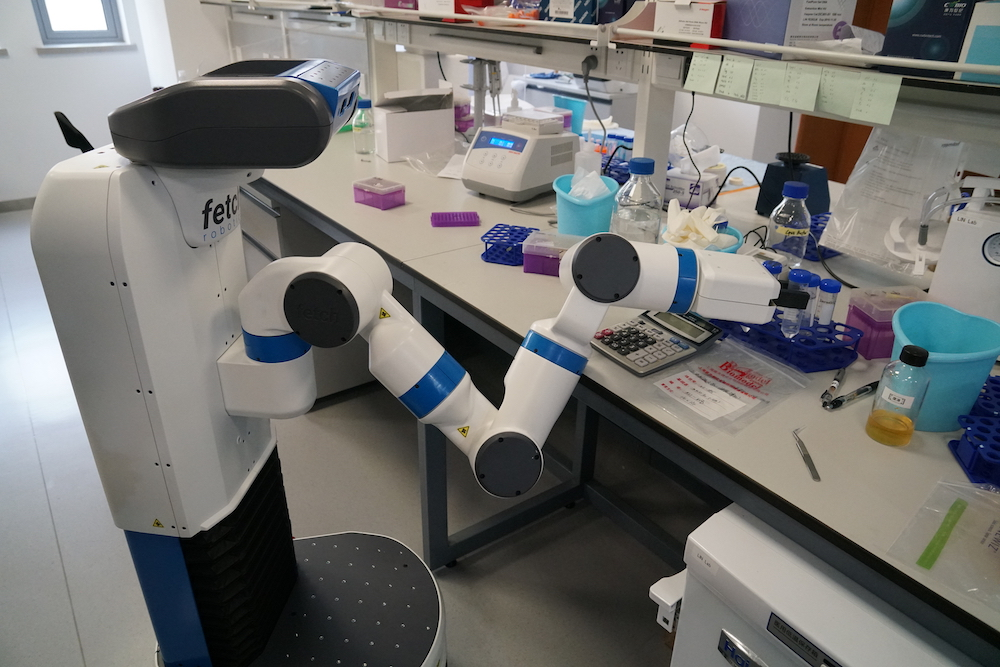
\includegraphics[width=0.75\textwidth]{img/robot.jpg}
		\caption{
			A mobile manipulation Fetch robot in the life science laboratory.
		}
		\label{robot}
	\end{figure}

	
	%\hfill mds
	%\hfill August 13, 2002
	
	\section{State of the Art}
	% The same requirements as the proposal (you have a chance to improve on the state of the art section – make sure that you follow the requirements thoroughly – read the proposal requirements again!) Additionally, present at least one more paper (in total, not per person) with at least 1/3 a page relevant to your problem.
	
	\subsection{JIAHUI}
	\subsubsection{Papers}
	In the last few years, there are a few works done on mobile manipulation as an integrated system and several mobile manipulators have been coming to the market, for example, Tiago by Pal Robotics, Mobile Baxter by Rethink Robotics, and Fetch and Freight by Fetch Robotics \cite{roa2015mobile}. 
	
	
	
	For labware transportation in life science laboratories, a mobile robot called H20 with dual arms capable of 6-Degree of Freedom (DOF) mobility, an indoor GPS navigation system and Kinect sensor developed by H. Liu. et al. \cite{liu2013mobile},\cite{ali2016kinematic} can realize manipulation tasks for different experimental objects such as flat panels and labware containers. However, different from general wheeled mobile manipulation, \cite{kim2018lab} proposes a lab automation drone and a robotic limb is attached to the robotic rotor-craft which could manipulate and transfer lines rapidly between test work-spaces. 
	
	\subsubsection{One further paper relevant to the project}
	In the paper\cite{olson2011apriltag}, they describe a method for robustly detecting visual fiducials and propose a graph-based image segmentation algorithm based on local gradients that allow lines to be precisely estimated. They specify and provide results on a set of benchmarks that will allow better comparisons of fiducial systems in the future. Their system is composed of two major components: the tag detector and the coding system.  
	\begin{itemize}
		\item Detection process\\
		The detector attempts to find four-sided regions that have a darker interior than their exterior. Tags are composed of black and white blocks similar to the QR code and different tags contain different ID information. First, paste some tags in the scene. Secondly, the gradient at every pixel is obtained, and then compute their magnitudes and direction. Using a graph-based method, pixels with similar gradient directions and magnitude are clustered into components. Using weighted least squares, a line segment is then fit to the pixels in each component. Once four lines have been found, a candidate quad detection is created. Finally, they compute the 3 $\times$ 3 homography matrix that projects 2D points in homogeneous coordinates from the tag’s coordinate system to the 2D image coordinate system. The homography is computed using the Direct Linear Transform (DLT) algorithm.
		\item Payload decoding\\ 
		The final task is to read the bits from the payload field. They do this by computing the tag-relative coordinates of each bit field, transforming them into image coordinates using the homography, and then thresholding the resulting pixels. In order to be robust to lighting (which can vary not only from tag to tag, but also within a tag), they use a spatially-varying threshold.
	\end{itemize}
	
	\subsubsection{ROS package}
	AprilTag is a free and open source visual fiducial system developed by the APRIL Robotics Laboratory of the University of Michigan, useful for a wide variety of tasks including augmented reality, robotics, and camera calibration. Targets can be created from an ordinary printer, and the AprilTag detection software computes the precise 3D position, orientation, and identity of the tags relative to the camera. The fiducial design and coding system are based on a near-optimal lexicographic coding system, and the detection software is robust to lighting conditions and view angles. 
	It uses a 2D bar code style “tag” similar to the QR code, allowing full 6-DOF localization of features from a single image.
	
	In this work, we used an open source ROS package apriltag\_ros for objects' pose estimation. The apriltag\_ros package is a ROS wrapper of the AprilTag 3 visual fiducial detection algorithm. Provides full access to the core AprilTag 3 algorithm's customizations and makes the tag detection image and detected tags' poses available over ROS topics (including tf). The core AprilTag 3 algorithm is extended to allow the detection of tag bundles and a bundle calibration script is provided (bundle detection is more accurate than single tag detection). Continuous (camera image stream) and single image detector nodes are available. The package works as shown in Fig. \ref{apriltag}. 
	
	
	\begin{figure}[H]  %%%f2
		\centering
		
\includegraphics[width=0.85\textwidth]{img/apriltag.png}
		\caption{
			Overview of the apriltag\_ros package.
		}
		\label{apriltag}
	\end{figure}
	
	
	\subsection{YIZHENG}
	% Deisenroth et al.\cite{deisenroth2011learning} proposed a Data-Efficient Reinforcement Learning method that allows low-cost manipulator to stacke blocks. 
	\subsubsection{Papers}
	
	Schmitt et al.\cite{8793824} propose a new model for sequential manipulation tasks that also considers robot dynamics and time-variant environments.
	It can automatically derive constraint-based controllers and use them as steering functions in a kinodynamic manipulation planner using this model.
	Thakar et al.\cite{8793501} propose an active learning based approach that can pick-up parts while the mobile base and the gripper are moving to minimize the operation time.
	
	Wang et al.\cite{Wang_2019_CVPR} propose a generic framework for estimating the 6D pose of a set of known objects from RGB-D images and deploy the proposed method to a real robot to grasp and manipulate objects based on the estimated pose.
	
	\subsubsection{One further paper relevant to the project}
	In this work, the author present DenseFusion, a generic framework for estimating 6D pose of a set of known objects from RGB- D images.
	DenseFusion is a heterogeneous architecture that processes the two data sources individually 
	and uses a novel dense fusion network to extract pixel-wise dense feature embedding, from which the pose is estimated.
	Furthermore, they integrate an end-to-end iterative pose refinement procedure that further improves the pose estimation 
	while achieving near real-time inference. 
	The experiments show that this method outperforms state-of-the-art approaches in two datasets, YCB-Video and LineMOD. 
	The method's architecture contains two main stages. 
	The first stage takes the color image as input and performs semantic segmentation for each known object category.
	Then, for each segmented object, feed the masked depth pixels (converted to 3D point cloud) as well as an image patch cropped by the bounding box of the mask to the second stage.
	The object pose is obtained by the second stage processes.
	It comprises four components:
	\begin{itemize}
		\item  a fully convolutional network that processes.
		\item a PointNet-based network that processes each point in the masked 3D point cloud to a geometric feature embedding.
		\item a pixel-wise fusion network that combines both embeddings and outputs the estimation of the 6D pose of the object based on an unsupervised confidence scoring.
		\item an iterative self-refinement methodology to train the network in a curriculum learning manner and refine the estimation result iteratively.
	\end{itemize}
	We will try to use this algorithm to estimate the centrifuge tube's pose and then grasp it. 
	
	\subsubsection{ROS package}
	The move\_base package provides an implementation of an action that, given a goal in the world, will attempt to reach it with a mobile base. The move\_base node links together a global and local planner to accomplish its global navigation task. 
	It supports any global planner adhering to the nav\_core::BaseGlobalPlanner interface specified in the nav\_core package 
	and any local planner adhering to the nav\_core::BaseLocalPlanner interface specified in the nav\_core package. 
	The move\_base node also maintains two costmaps, one for the global planner, 
	and one for a local planner that are used to accomplish navigation tasks.
	The pip line of the package is shown in Fig. \ref{movebase}
	\begin{figure}[H]    %%%f3
		\centering
		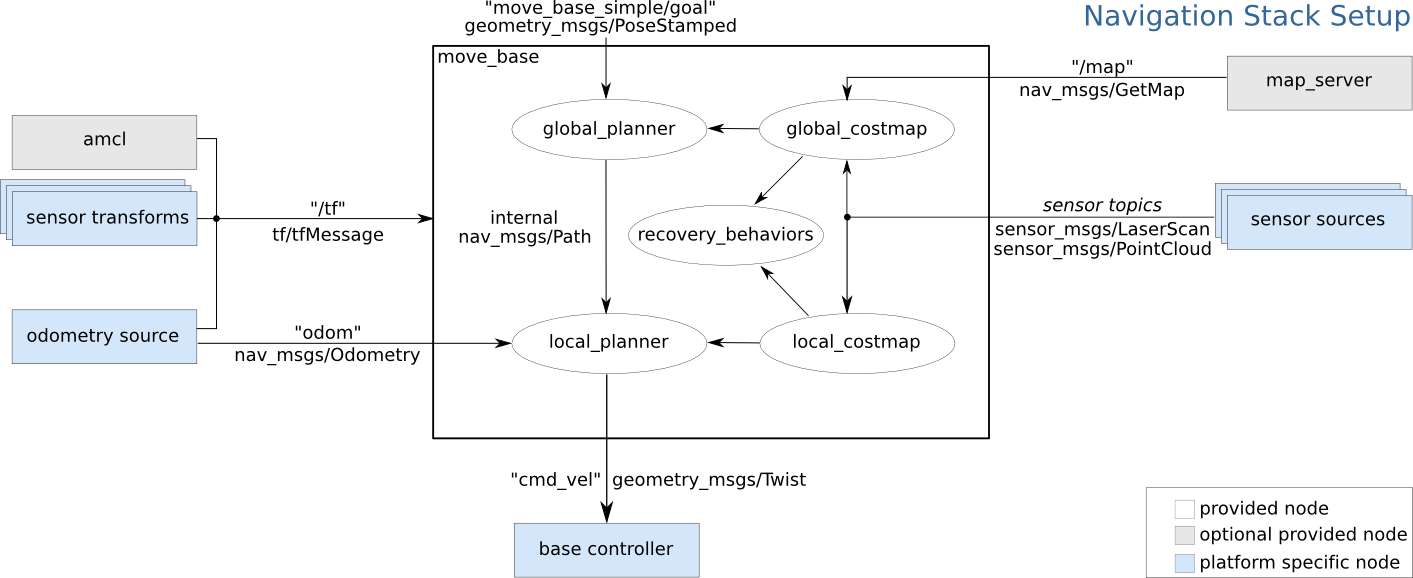
\includegraphics[width=0.9\textwidth]{img/movebase.png}
		\caption{
			The framework of the move base node.
		}
		\label{movebase}
	\end{figure}
	
	\subsection{Fetch robot}   
	In this project, we use the Fetch robot \cite{wise2016fetch} which is a mobile manipulator consisting of a differential drive mobile base, an arm with 7 degrees of freedom and 6kg payload, a pan and tilt head, a torso lift actuator, and a standalone mobile robot platform, as shown in Fig.\ref{overview}. The mobile base includes a SICK laser scanner with a 220-degree field of view and a 25-meter range. Freight also includes a base-mounted 3D camera. Fetch includes a head-mounted depth camera. The gripper is a modularity point, allowing custom grippers to be swapped in, but supplied with a default parallel-jaw gripper capable of grasping a wide range of objects. Intel-based computers provide processing power for navigation, manipulation and perception activities, while extensive battery capacity gives each robot an 8- to 10-hour run time.
   
    \begin{figure}[htbp] %%%f4
		\centering
		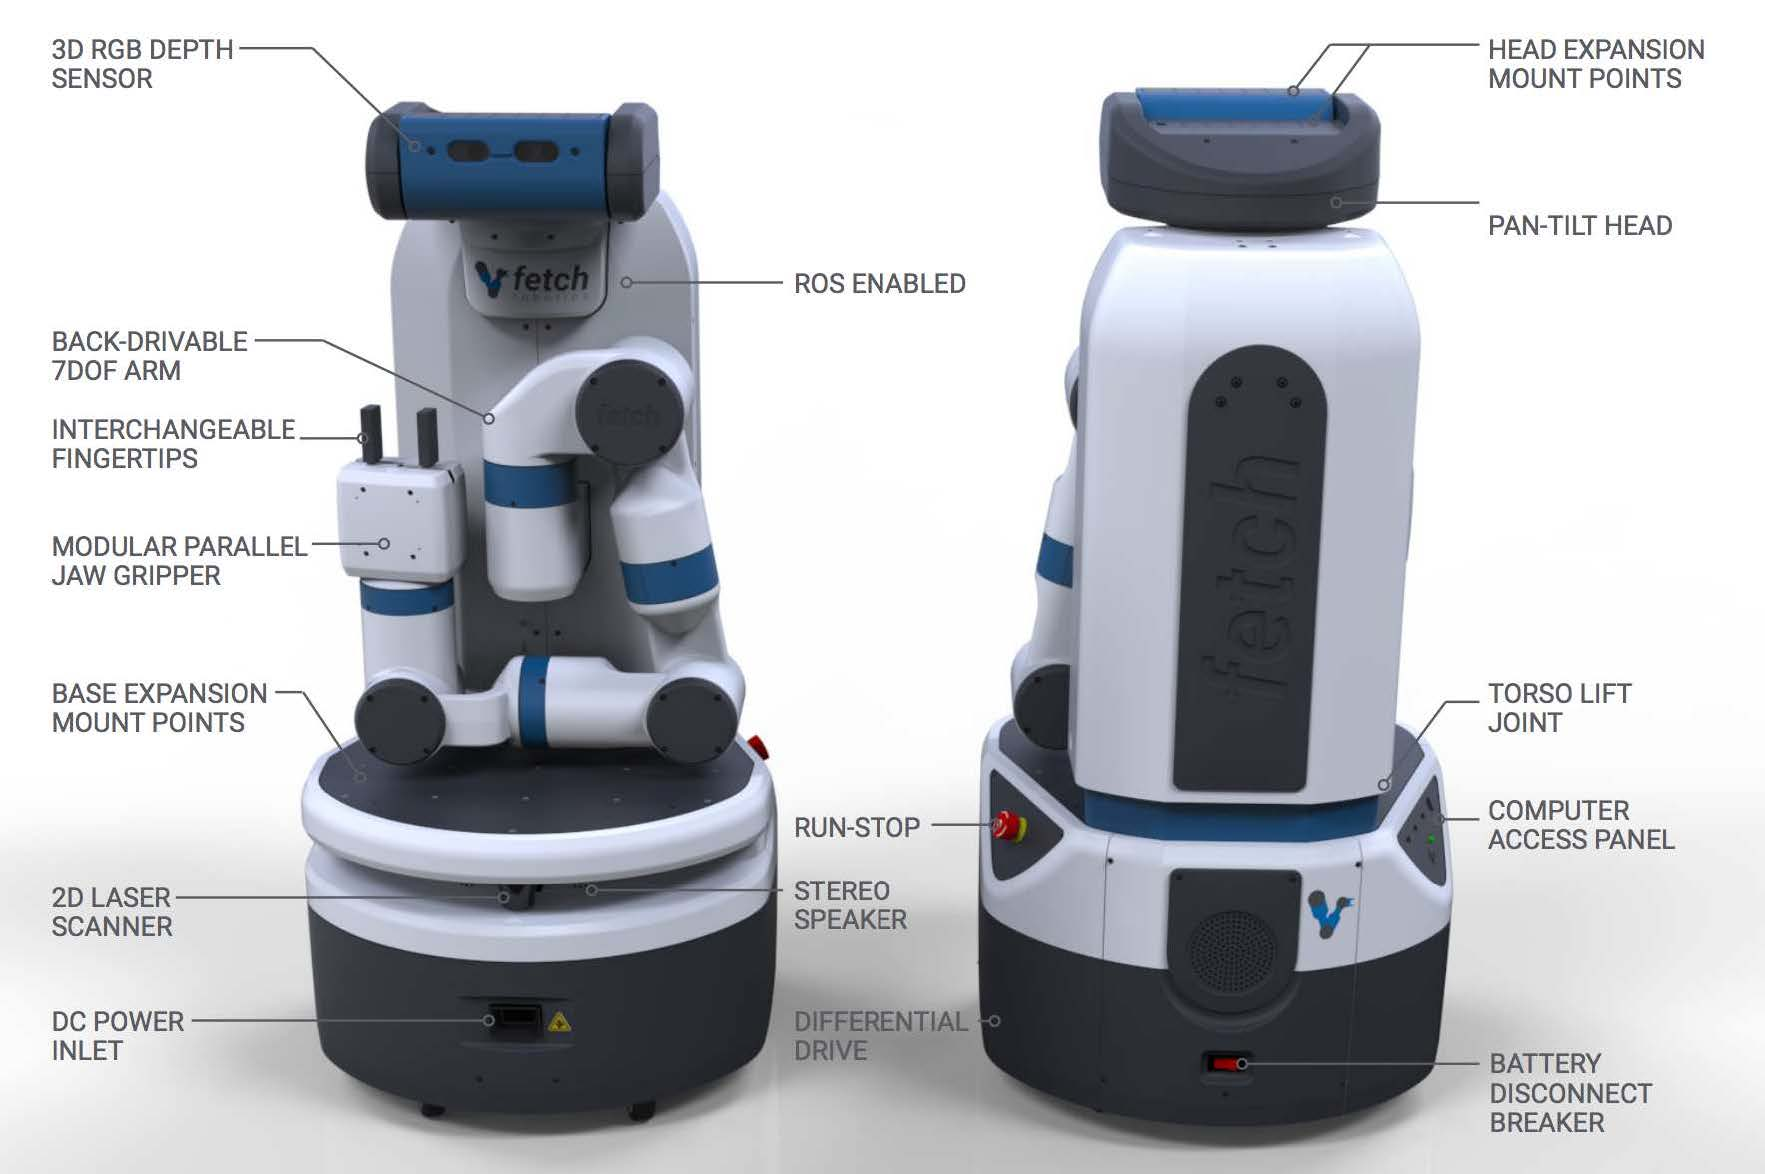
\includegraphics[width=0.8\textwidth]{img/FetchRobot.jpg}
		\caption{
			Overview of the Fetch robot.
		}
		\label{overview}
	\end{figure}
	
	
	\section{System Description}
	%Describe your idea and system & algorithm in detail. Also write which problems you overcame. Also add a subsection describing your ROS packages and code in some detail (at least one page). Make sure you have an image of your hardware (if so) –identifying all the important parts.
	The system contains 6 components:
	\begin{itemize}
		\item  MoveIt framework that is used to control the manipulator to grasp the object.
		\item Cartographer algorithm to build a map.
		\item Move base ros package that is used to navigate the robot to the target place where the object should be grasped.
		\item AprilTag 3 visual fiducial detection algorithm is used to obtain the object pose.
		\item We will try to implement DenseFusion framework to estimate the object pose to replace the AprilTag 3 algorithm since this algorithm does not need to add the QR code on the object we want to grasp.
		\item We will design a device that can clamp for test tubes on the robot.
	\end{itemize}
	
	\begin{figure}[htbp] %%%f5
		\centering
		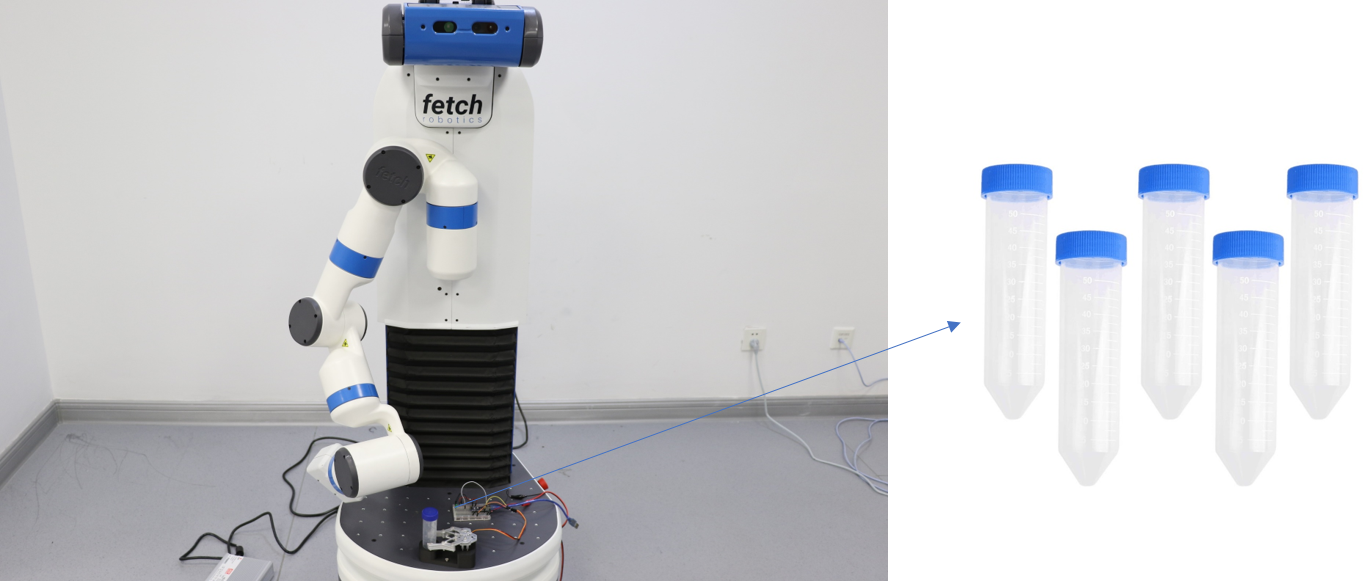
\includegraphics[width=0.9\textwidth]{img/fetch.png}
		\caption{
			Hardware of the experiment and centrifuge tubes with screw lid.
		}
		\label{tube}
	\end{figure}
	
	
	Firstly, we put the AprilTag on the tubes. Once the camera sees the AprilTag, the pose of the tube is obtained and we set the coordinate
	as the goal of the inverse kinematics. The manipulator reaches directly above the object, then drops vertically to grab it. 
	After the tube is grasped, the manipulator places the tube on the device mounted on the robot,
	and then unscrew the lid from the top of the centrifuge tube (Fig. \ref{tube}) and place it on the test table.
	Now we can add something into the tube if needed.
	The manipulator re-position the lid, grasp and re-screw it. 
	Also, we use cartographer, a graph-based SLAM algorithm to build the map of the lab. And then use this map to navigate our robot 
	to the test table through move base ros package.
	
	\subsection{Actionlib software interface}
	Fetch Robot contains three actionlib services:
	\begin{itemize}
	\item \/gripper\_controller/gripper\_action: it can control the gripper open or close.
	\item \/gripper\_controller/led\_action: there are four led on the gripper, we can control the status of the led to represent the status of the robot.
	\item \/head\_controller/point\_head: it can control the head of the robot that decide where the robot look at.
	\end{itemize}
	
	
	\subsection{Using MoveIt framework to control the manipulator to grasp the object}
	Fetch Robot contains three moveit groups:  
	\begin{itemize}
	\item 7 DOF robot arm.
	\item 7 DOF robot arm with torso.
	\item Gripper.
	\end{itemize}
	
	The gripper group an alternative method to control the gripper, the more often used method is the actionlib method.
	For the most time, 7 DOF robot arm moveit group already can meet our needs to grasp the object. Torso is needed when we want the robot to grasp something high.
	
	\begin{figure}[htbp]  %%%f6
		\centering
		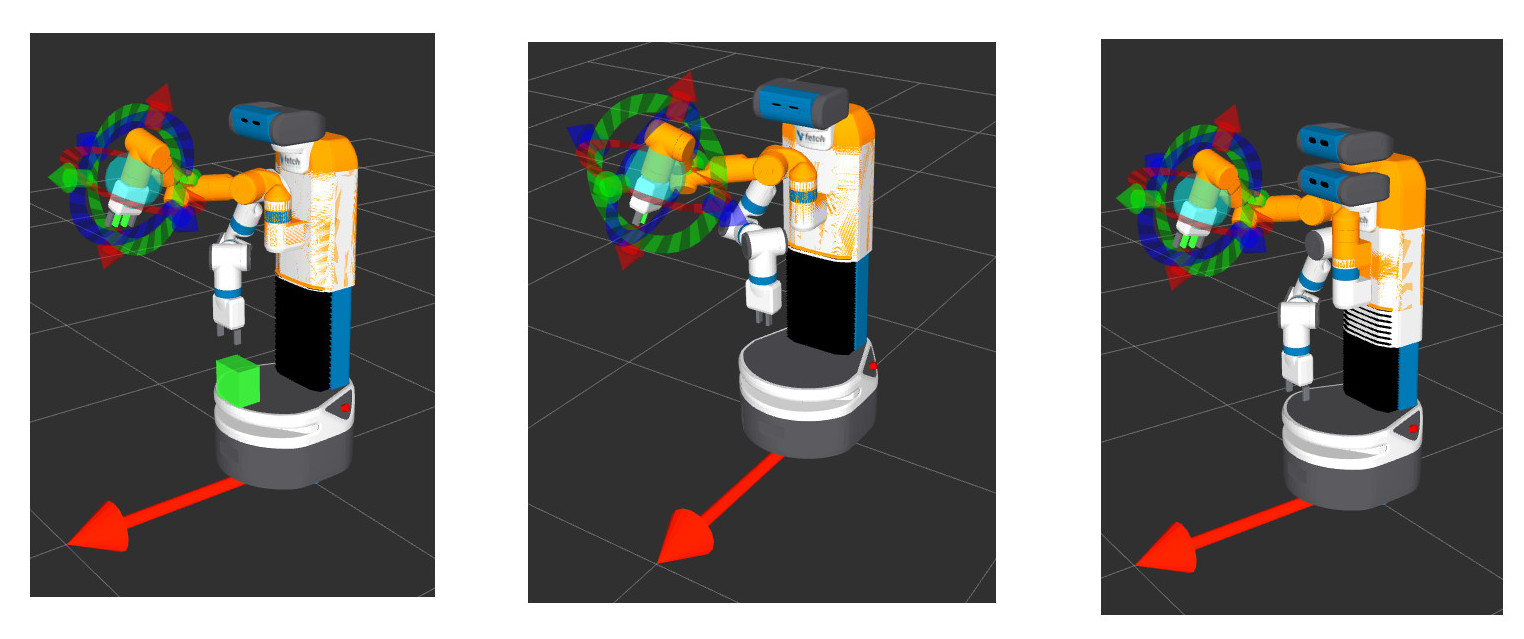
\includegraphics[width=0.9\textwidth]{img/rviz.jpg}
		\caption{
			The process of grasping the tube.
		}
		\label{rviz}
	\end{figure}
	
	\begin{figure}[b]  %%%f7
    \centering
    \subfigure[Gripper clamping]{ \label{a}
    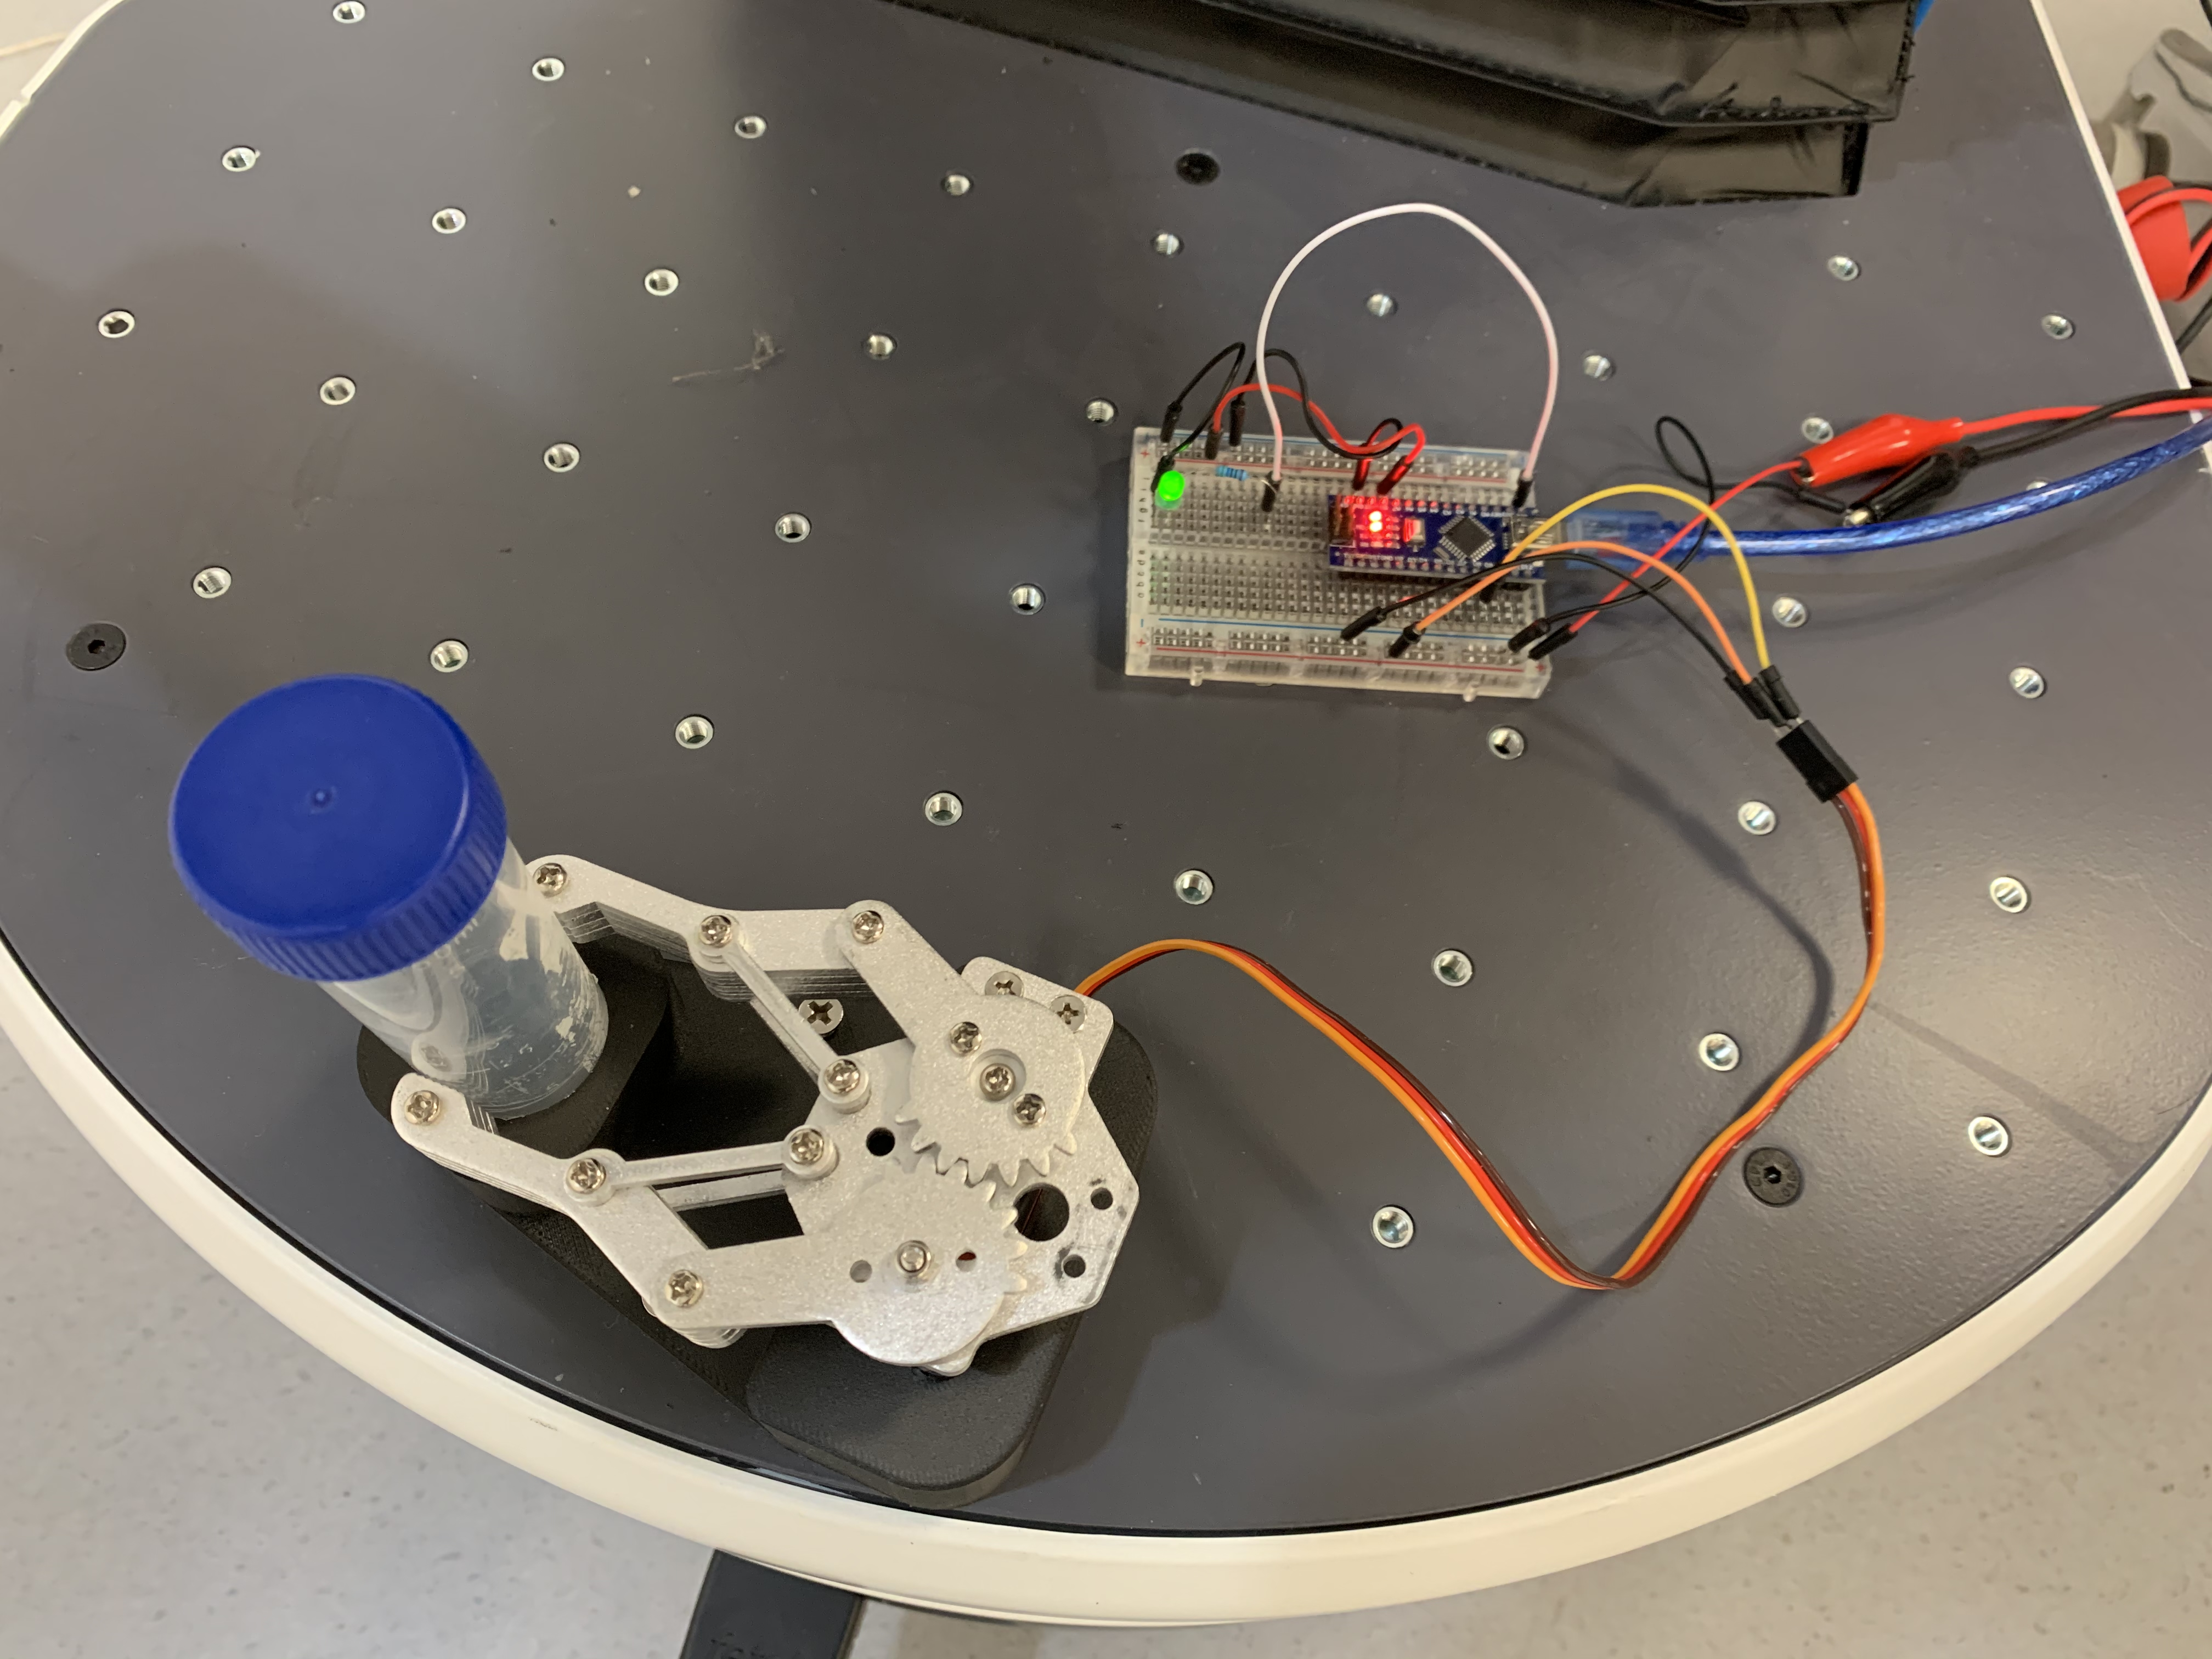
\includegraphics[width=0.43\textwidth]{img/s1.jpg}
    }
    \subfigure[Gripper releasing]{ \label{b}
    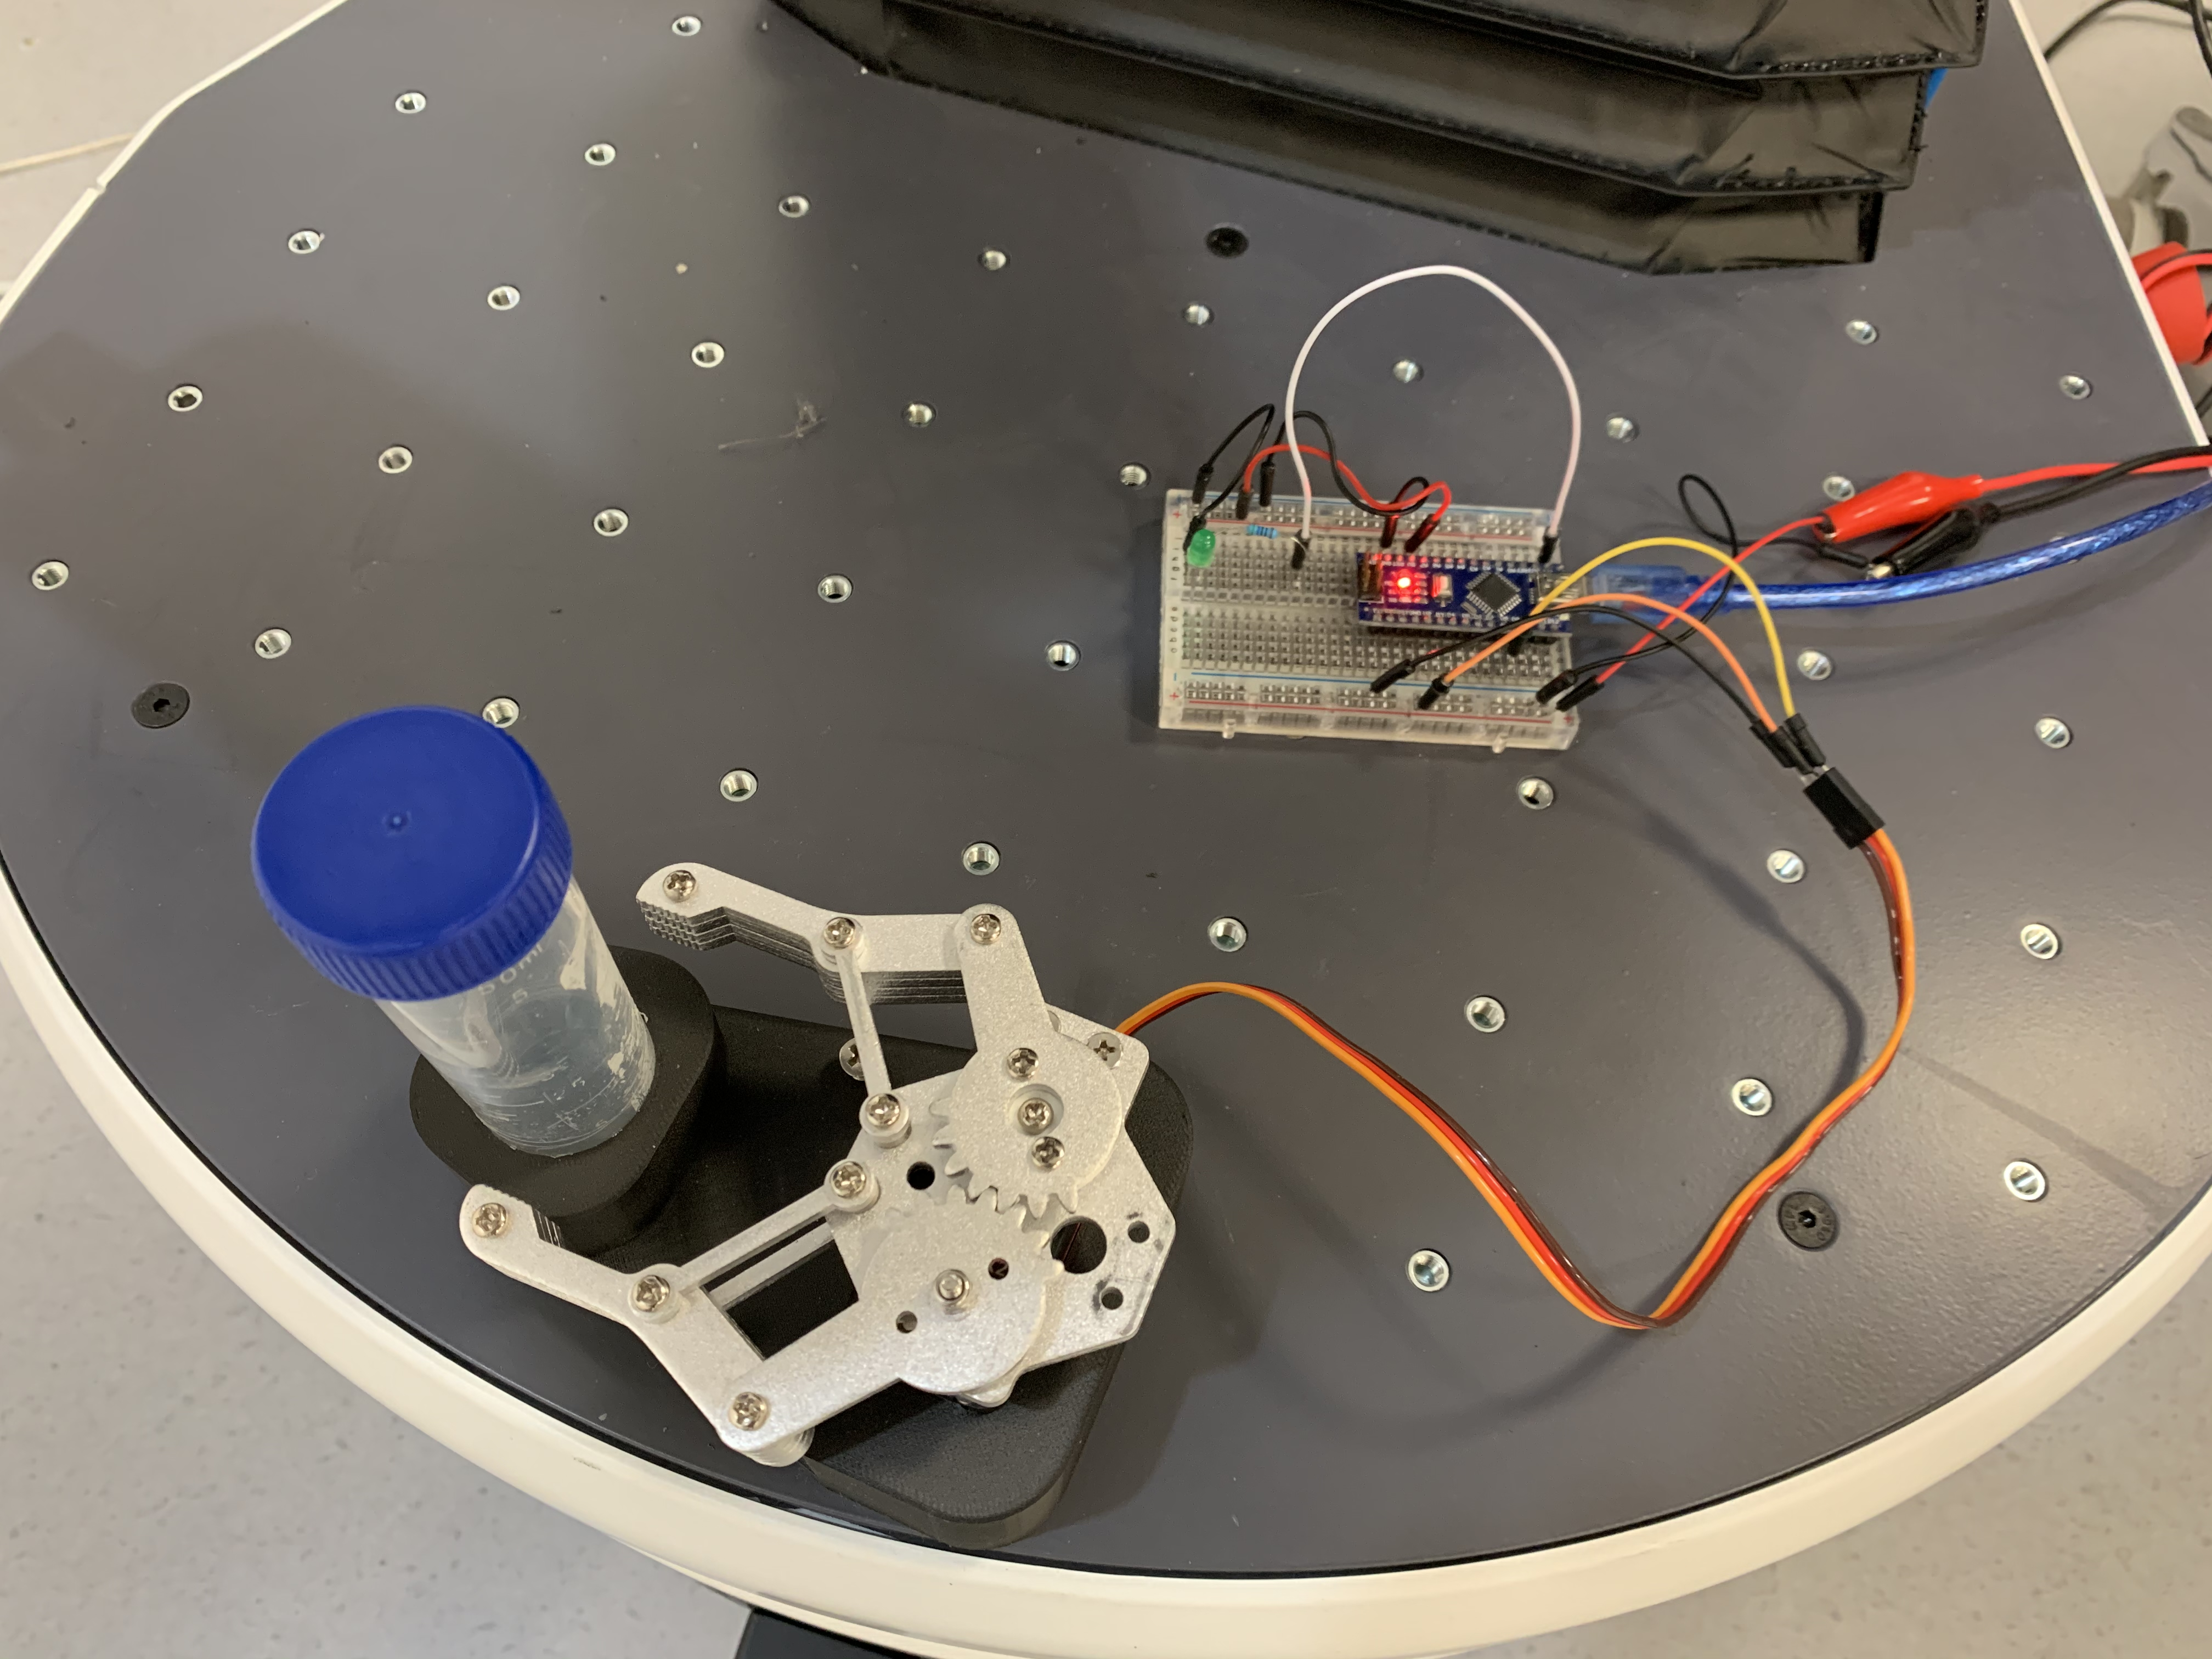
\includegraphics[width=0.43\textwidth]{img/s2.jpg}
    }
    \caption{The fixture and the arduino board are mounted on the base of Fetch.}
    \label{fixture}
    \end{figure}
    
	The process of grasping the tube:
	The arm firstly should move on top of the fixture and then move down to place the test tube into the fixture.
	Since we install a fixture on top of the robot base, it is required to consider the collision between the robot arm and the fixture into account when the arm is planning the trajectory. So there is a collision object named "fixture" being added to the moveit PlanningSceneInterface. See Fig. \ref{rviz} left.
	After the arm is on top of the fixture, the only requirement of the arm is moving down. It only need one freedom movement, so we decide to move the torso, 7 DOF robot arm with torso moveit group is used to do this work. On the other hand, the test tube attitude does not allow rotation, so it has to add the orientation constrain when the arm is planning. We use moveit\_msgs::Constraints to add the constraints to the moveit. The quaternion is set as (x:0.707, y:0, z:-0.707, w:0) to keep the gripper face down. See Fig. \ref{rviz} middle.
	
	After the arm moves down, the robot can rotate the last joint to screw the lid. It also needs moveit to finish. The trajectory is planned in the joint space. A sequence of the desired angle is sent to make the joint rotate. But maybe due to the framework bug, in this part, the robot can not plan successfully.
	
	\subsection{Fixture design of the centrifuge tube}
    The fixture of the centrifuge tube contains two parts, a clamping part, and a fixed part. The gripper is controlled by the servo to clamp and release, as shown in Fig.\ref{fixture} and the servo library of arduino can be used to easily control the stroke and speed of the servo. Considering that the gripper and the centrifuge tube need to be mounted on the platform of Fetch, we used SolidWorks 3D modeling software to design a base that can hold the centrifuge tube and the gripper, and then we printed it with a 3D printer. Finally, we bolted the entire fixture to the mobile robot platform.
	
	\subsection{Communicate between Fetch and the fixture using rosseiral ROS package}
	Rosserial is a protocol for wrapping standard ROS serialized messages and multiplexing multiple topics and services over a character device such as a serial port or network socket. It contains several client libraries allowing users to easily get ROS nodes up and running on various systems. In our case, we use a arduino board to control the fixture, the rosserial\_arduino is used in our case. There is a subscribe node running in arduino which subscribe the command from the robot. It is a trigger information so an empty message already meets our needs. When the robot arm picks the tube on top of the fixture, the robot sends an empty message to trigger the fixture to fix the tube.
	
    
	
	\section{System Evaluation}
	%Describe how you want to test (final: tested) test your system. Most likely you will make some experiments – describe them here. At least show some first results. Very important: Also come up with measures that you define “what is a successful system”. For example: pick up in total 3 objects within 10 minutes. Or: Drive “full speed” for 10 minutes along a square with some people traffic without crashing.
	This work aims to use the Fetch robot for grasping and placing the centrifuge tube where the desired labware is positioned. Due to the centrifuge tube has a lid, we need to use the Fetch robot's parallel grippers to unscrew and re-screw the lid. Thus, we conducted several experiments, as shown in Fig.\ref{movement}.
	
	\begin{figure}[htbp]  %%%f8
    \centering
    \subfigure[Original position]{ \label{a}
    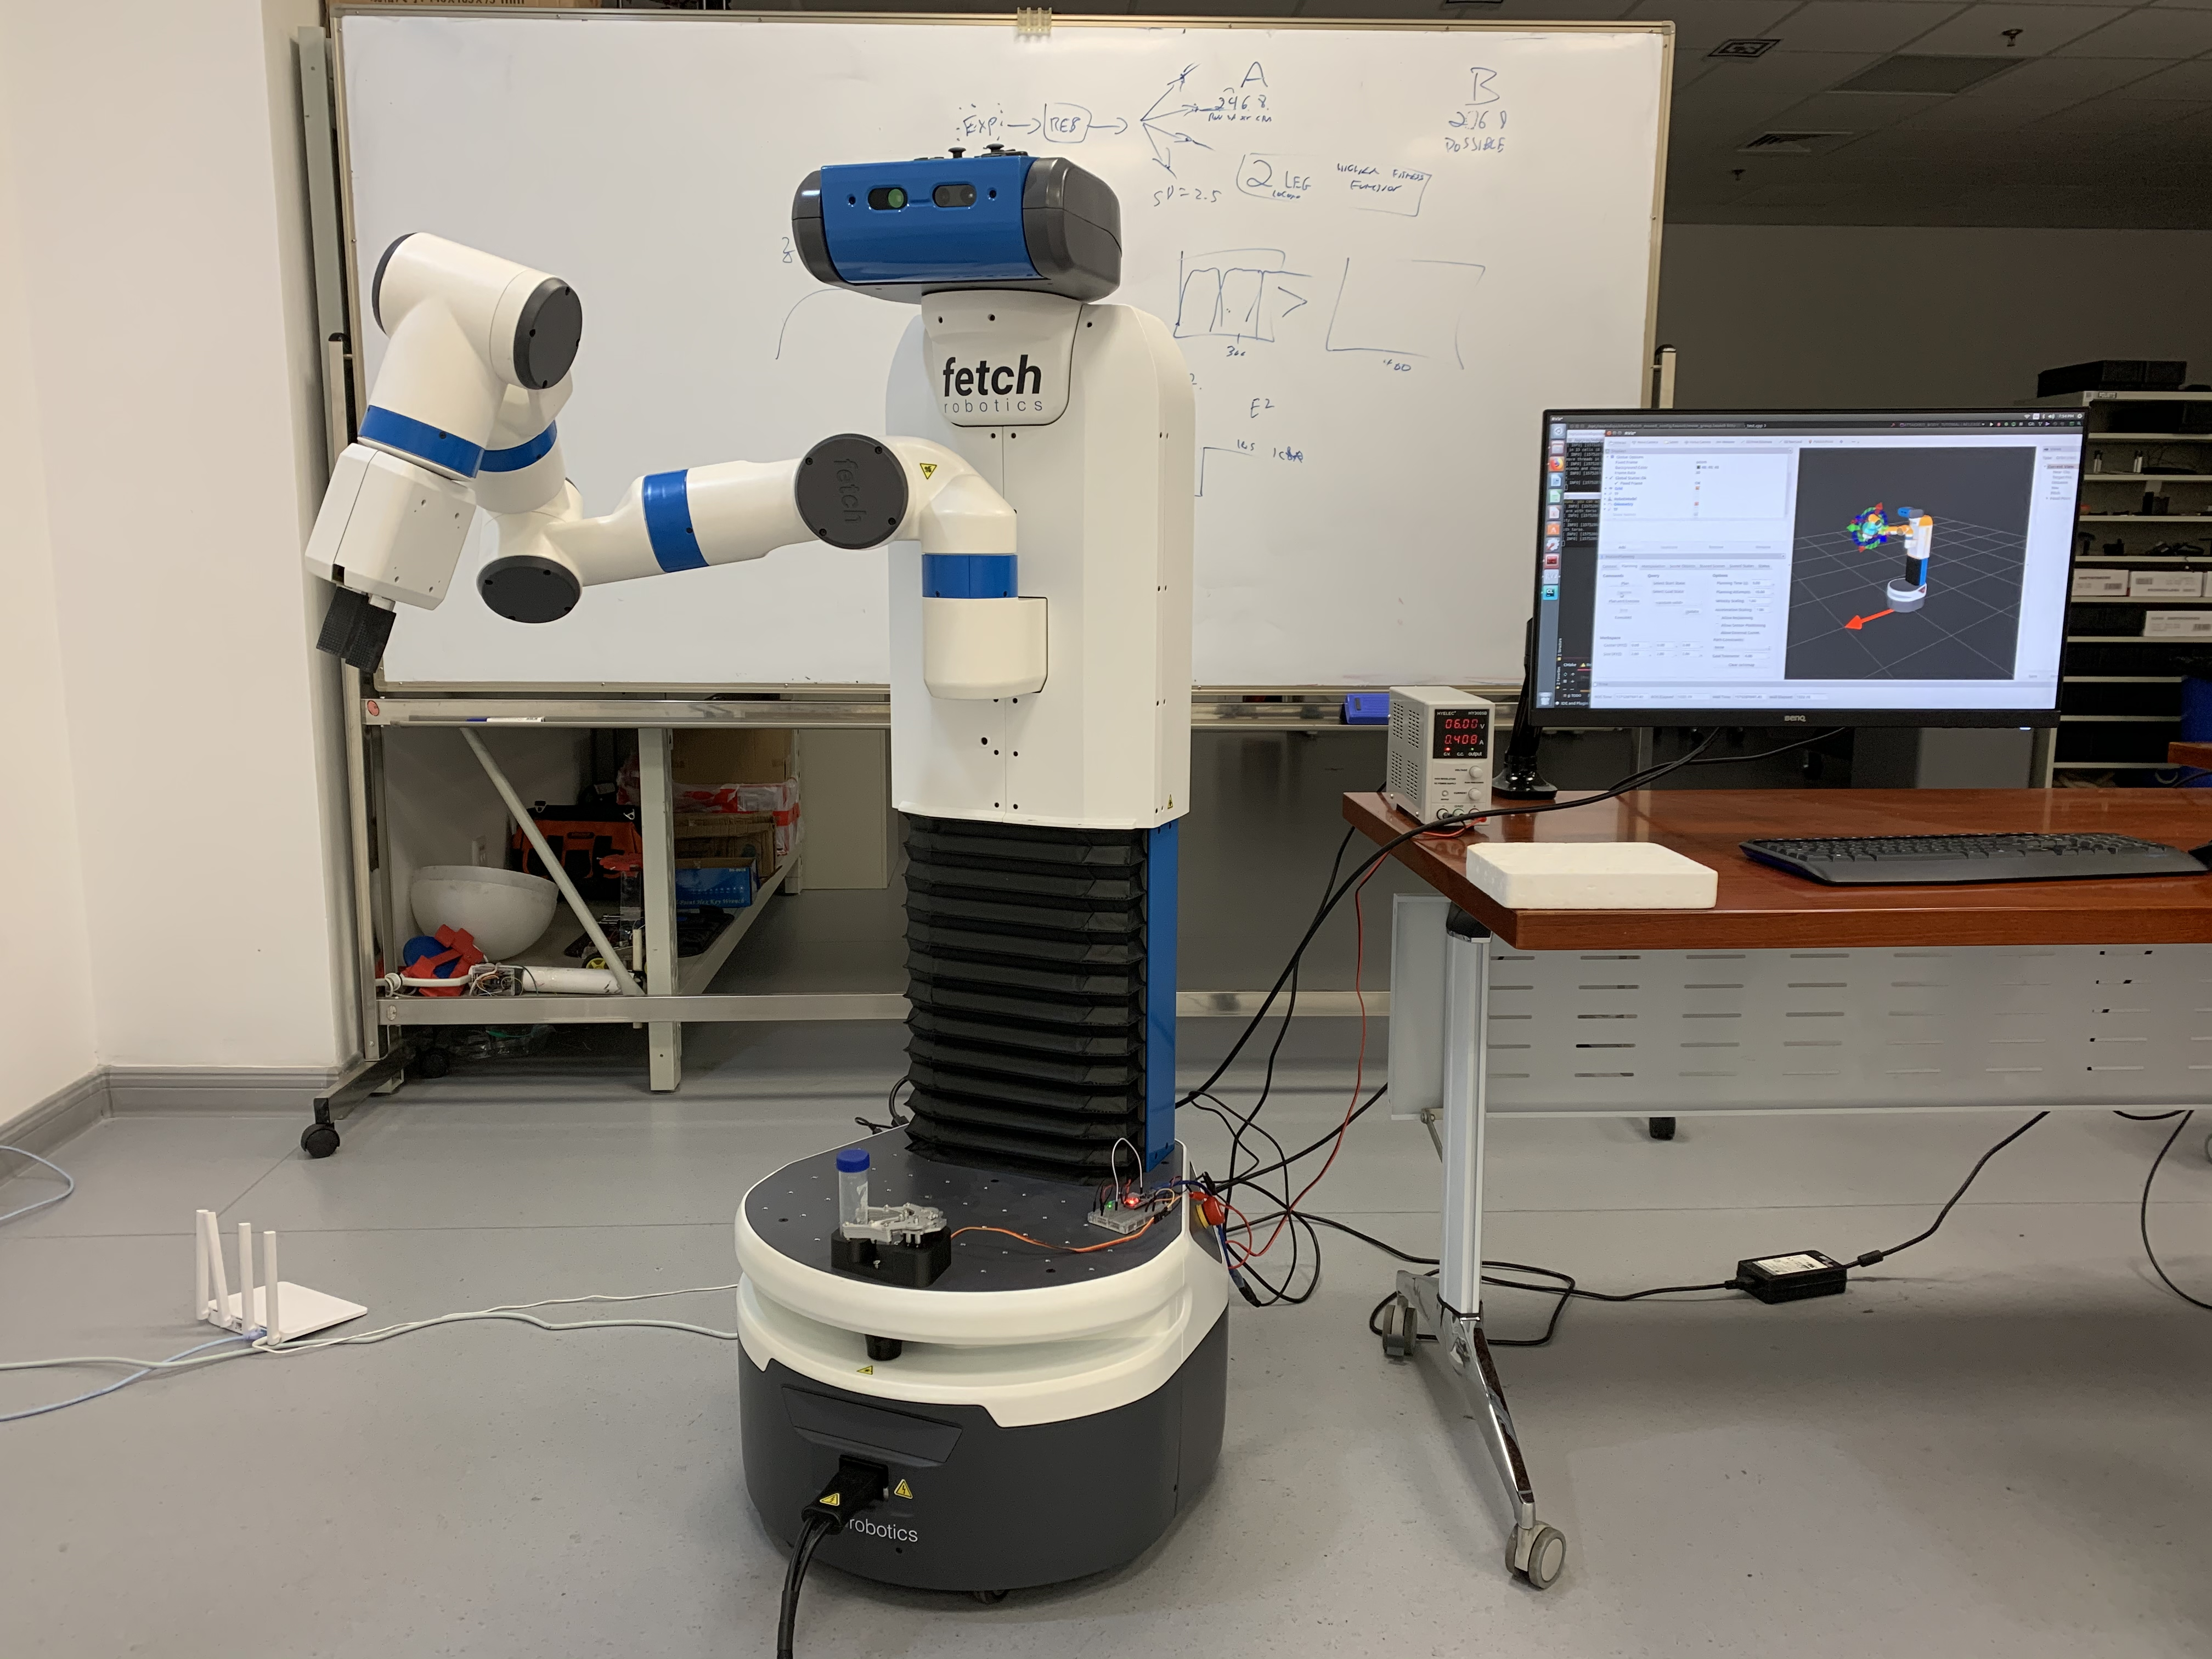
\includegraphics[width=0.3\textwidth]{img/p1.jpg}
    }
    \subfigure[Manipulator moving on top of the fixture]{ \label{b}
    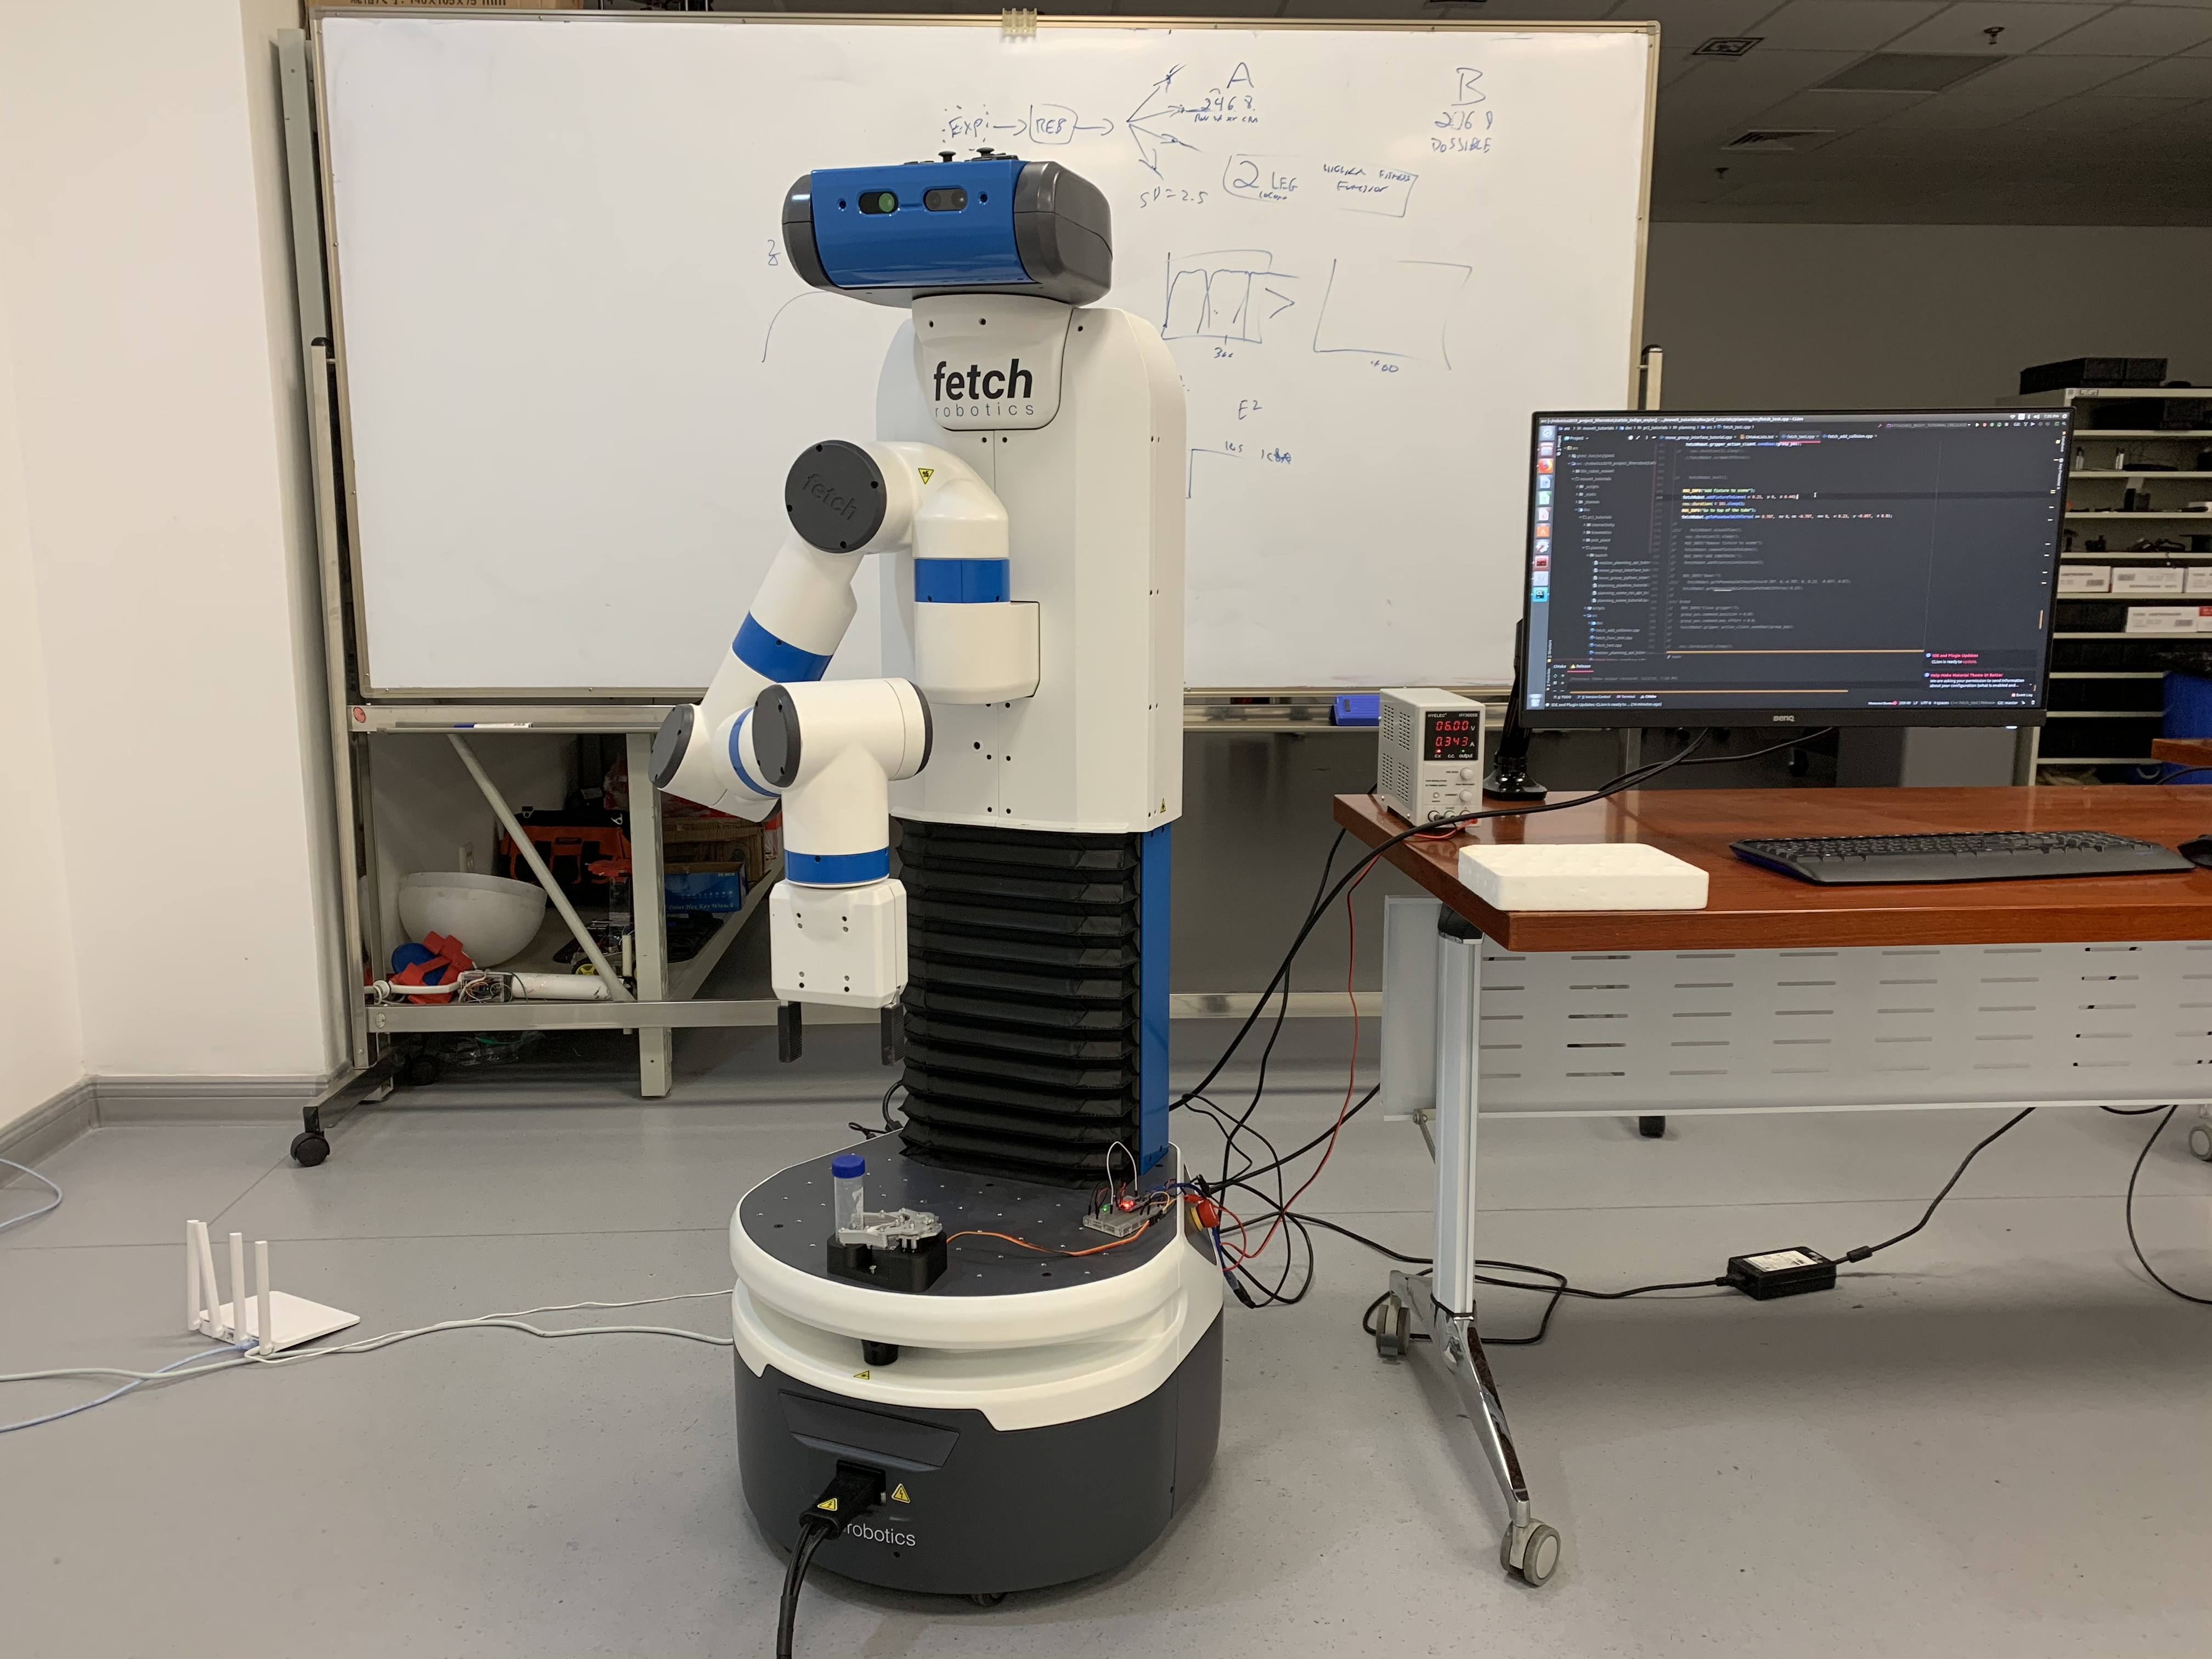
\includegraphics[width=0.3\textwidth]{img/p2.jpg}
    }
    \subfigure[Torso going down]{ \label{c}
    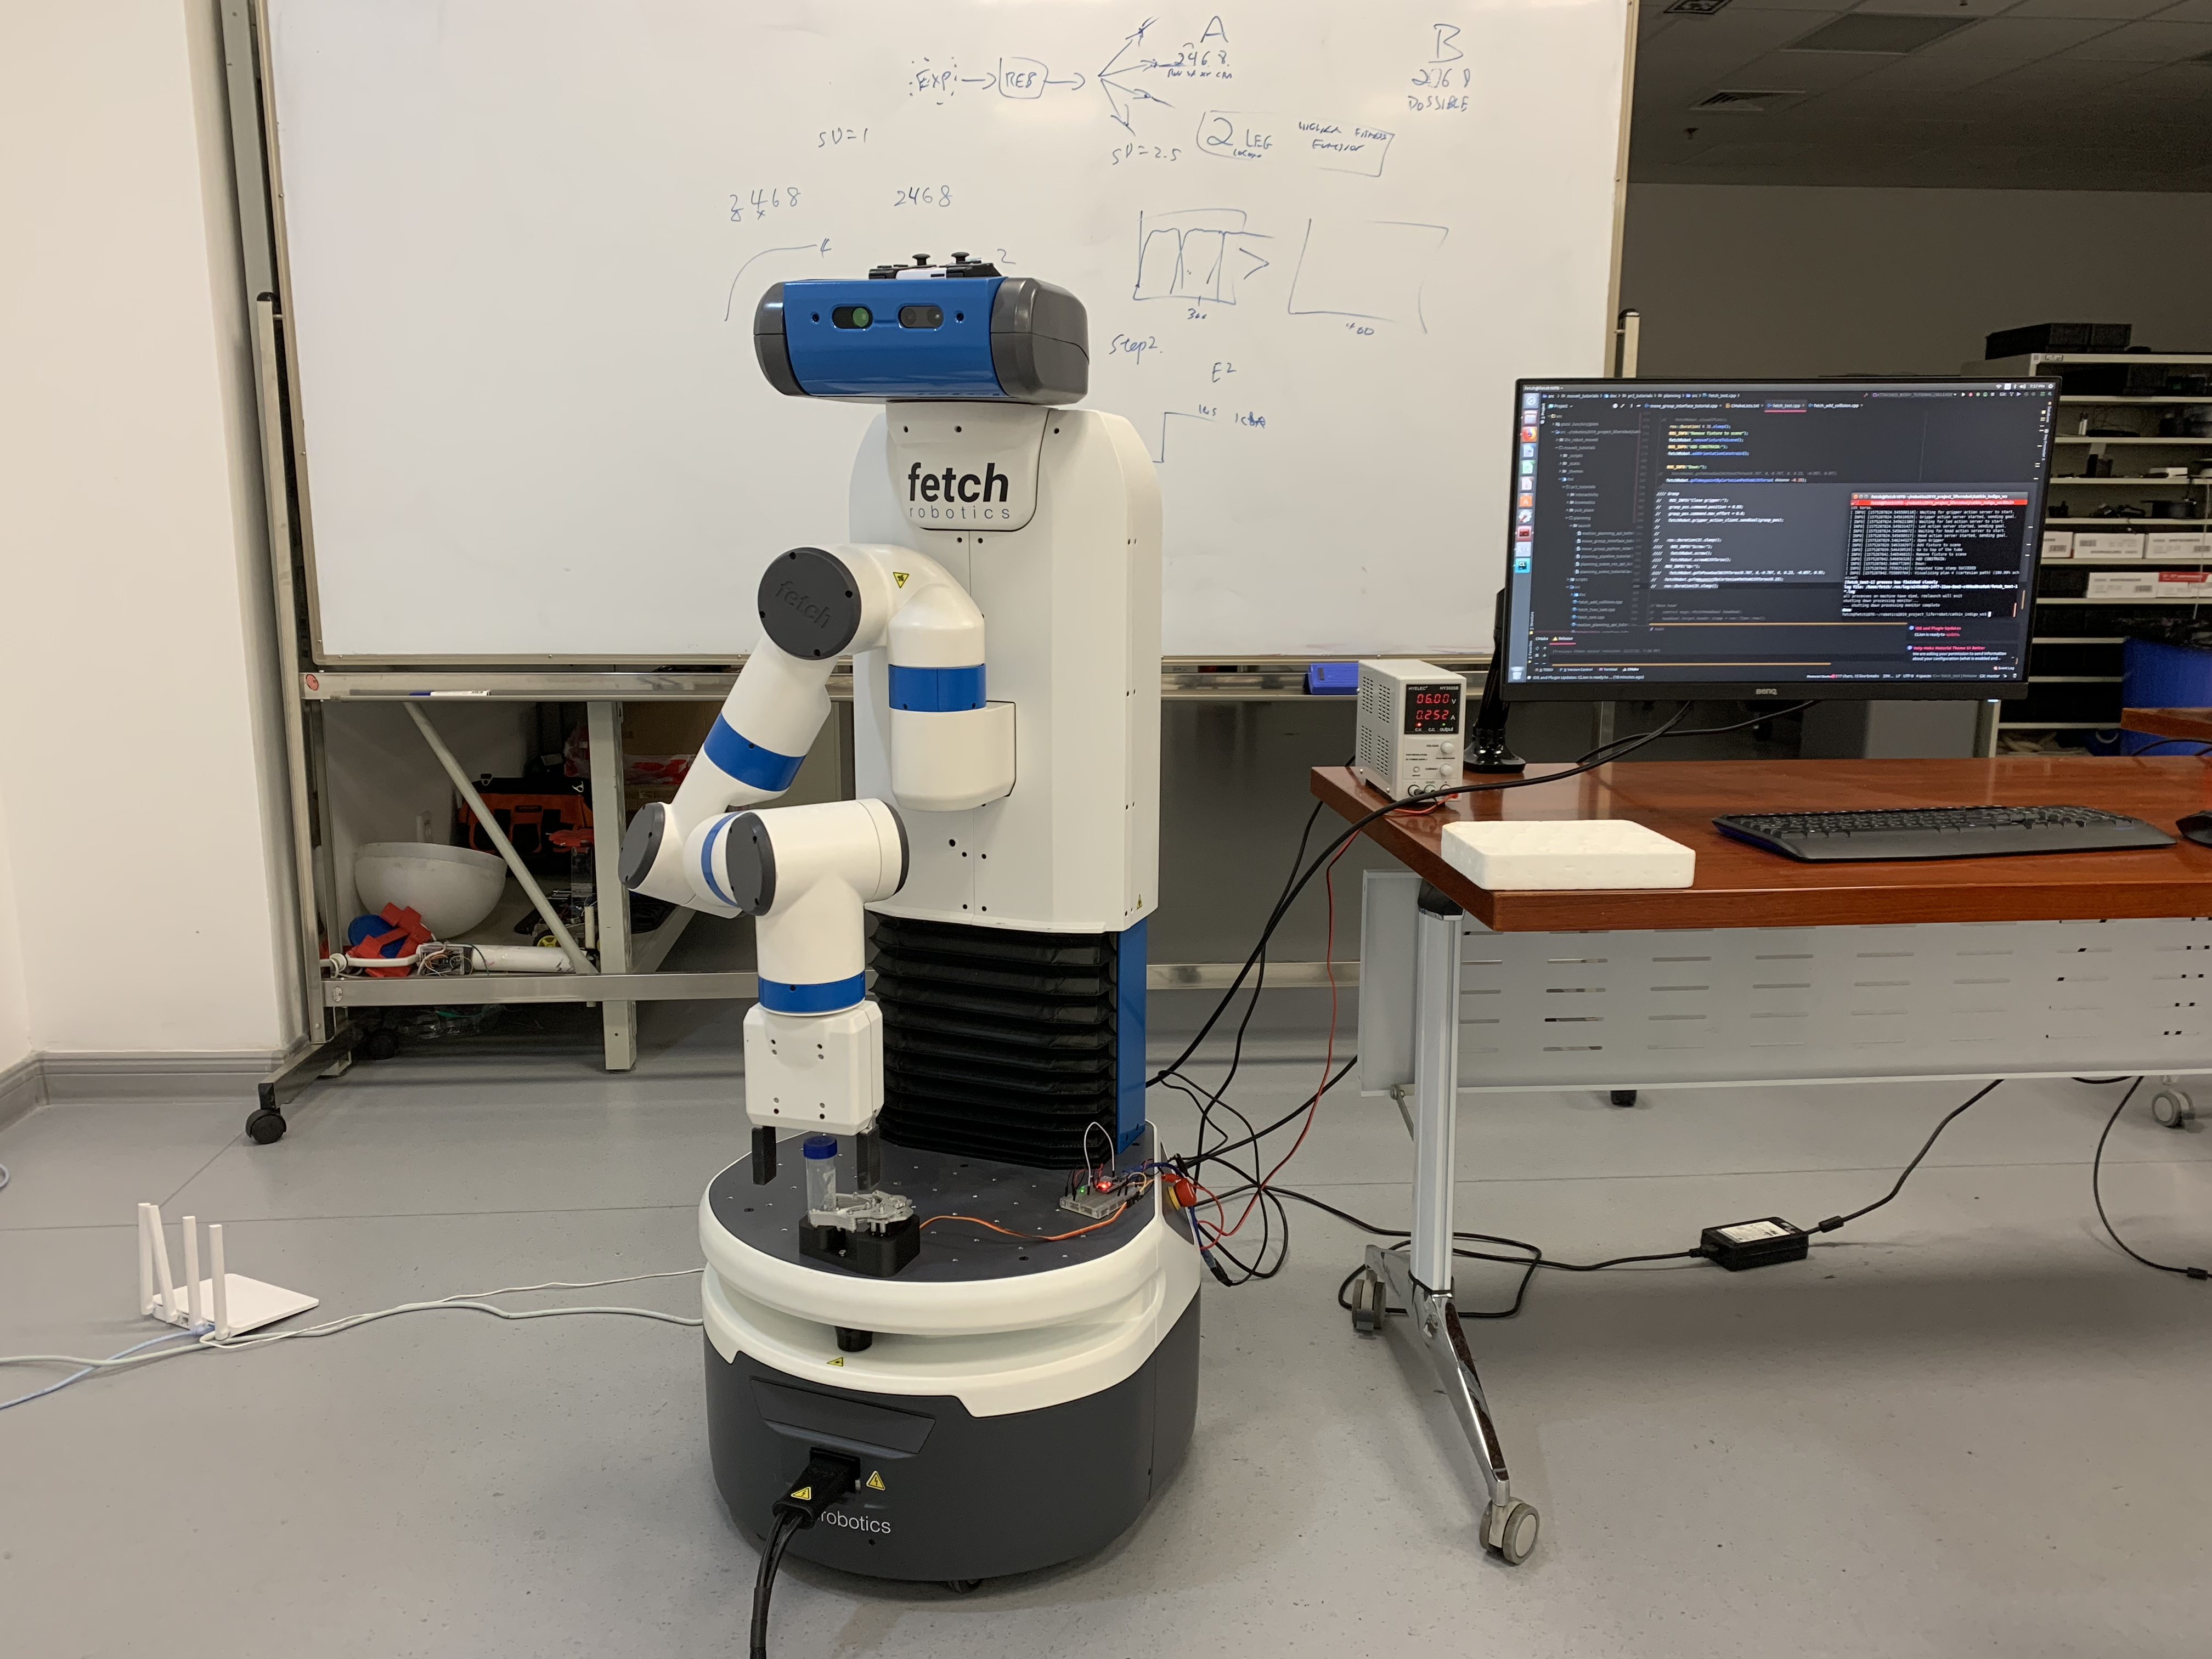
\includegraphics[width=0.3\textwidth]{img/p3.jpg}
    }
    \quad
    \subfigure[Parallel-jaw gripper grasping the tube]{ \label{d}
    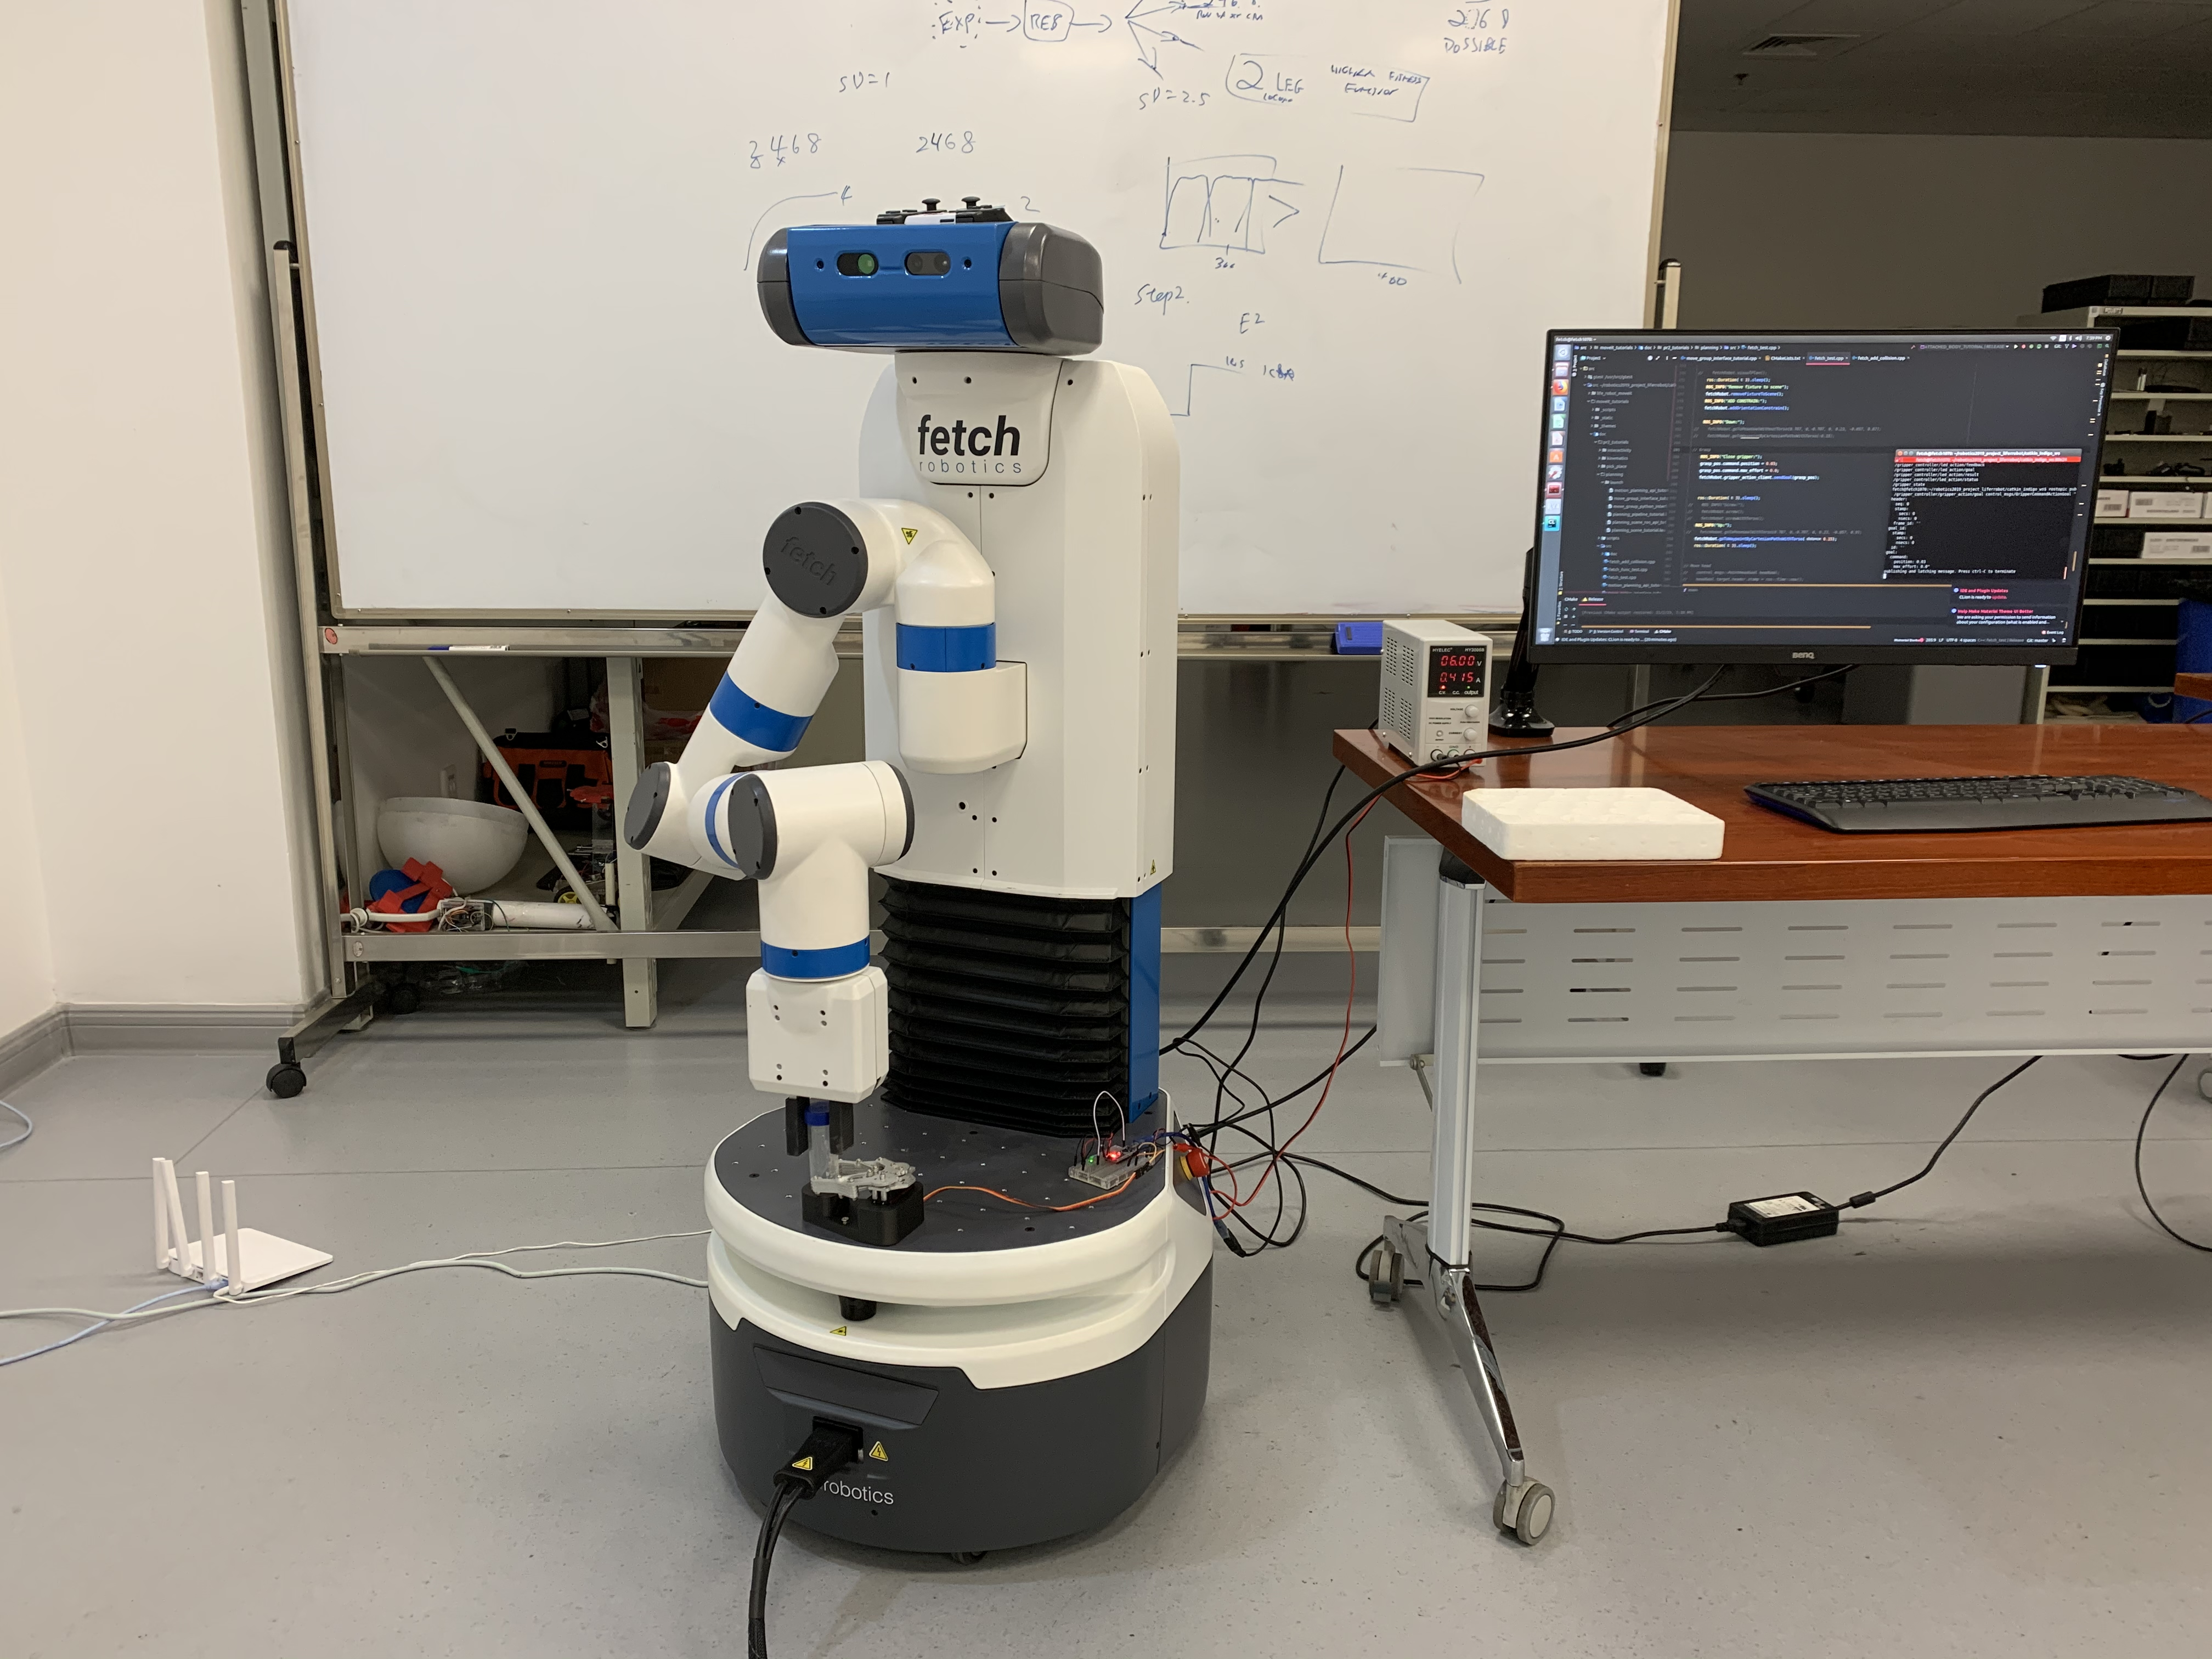
\includegraphics[width=0.3\textwidth]{img/p4.jpg}
    }
    \subfigure[Fixture releasing]{ \label{e}
    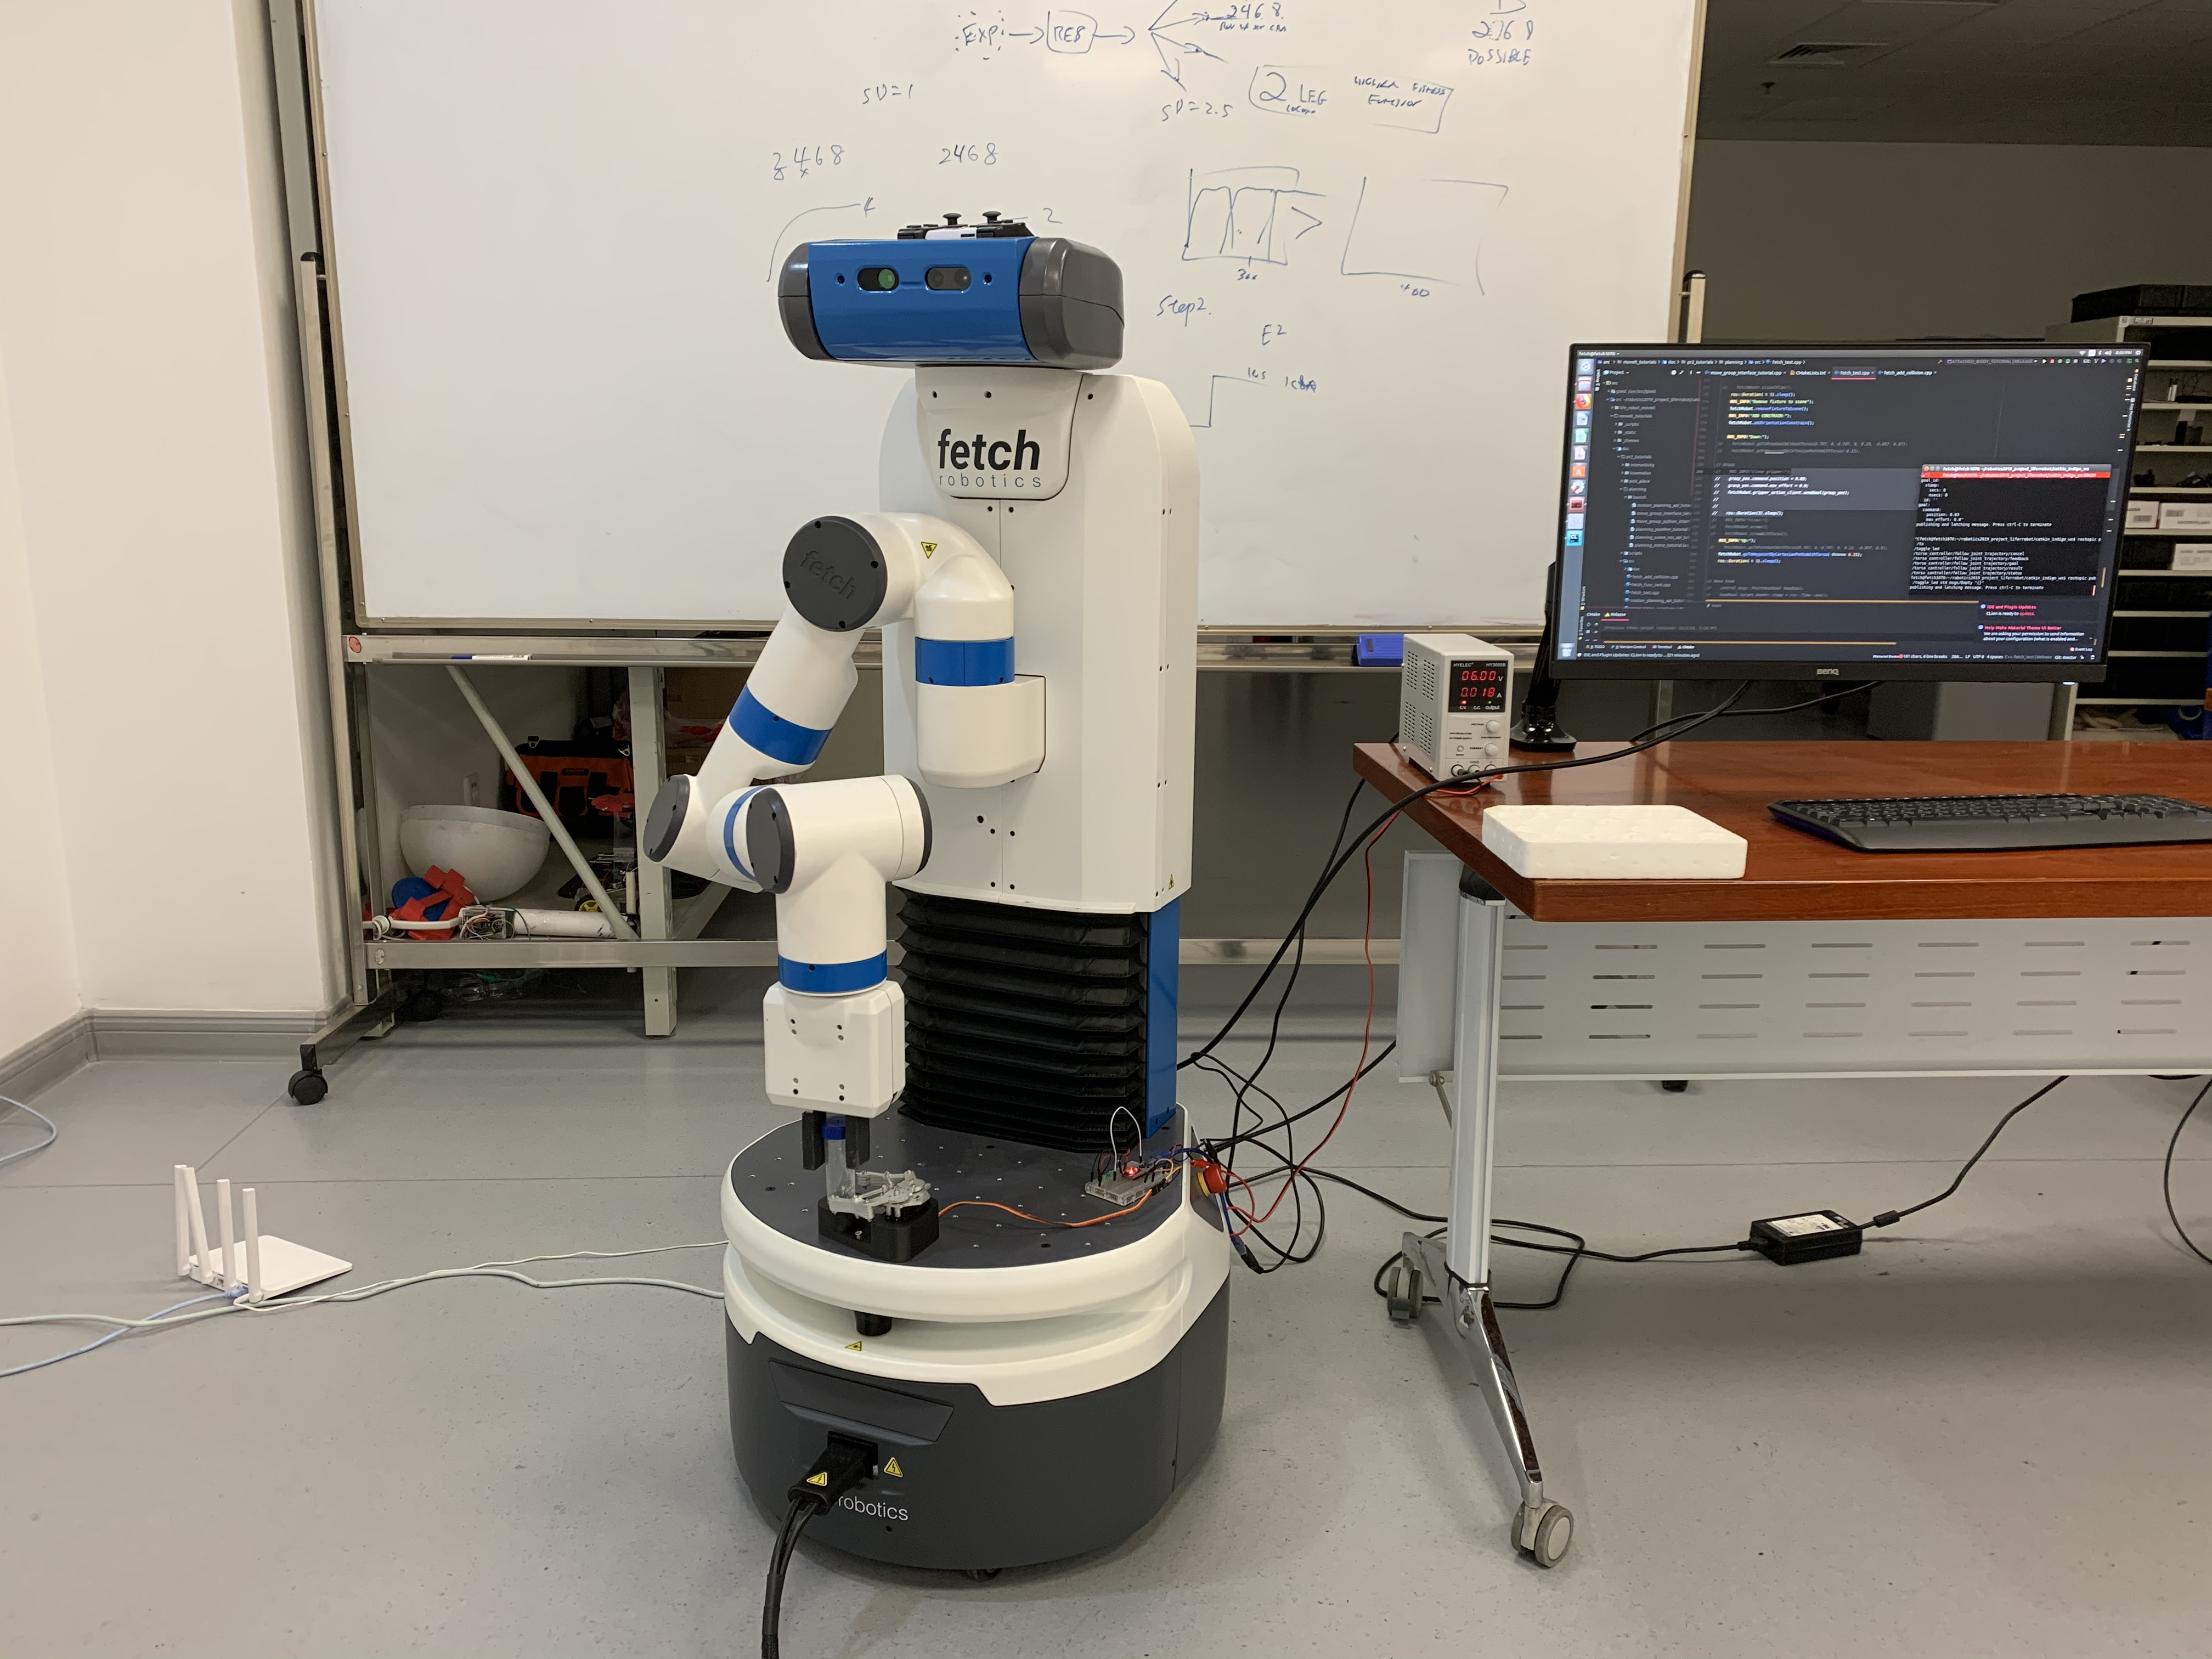
\includegraphics[width=0.3\textwidth]{img/p5.jpg}
    }
    \subfigure[Torso lifting up]{ \label{f}
    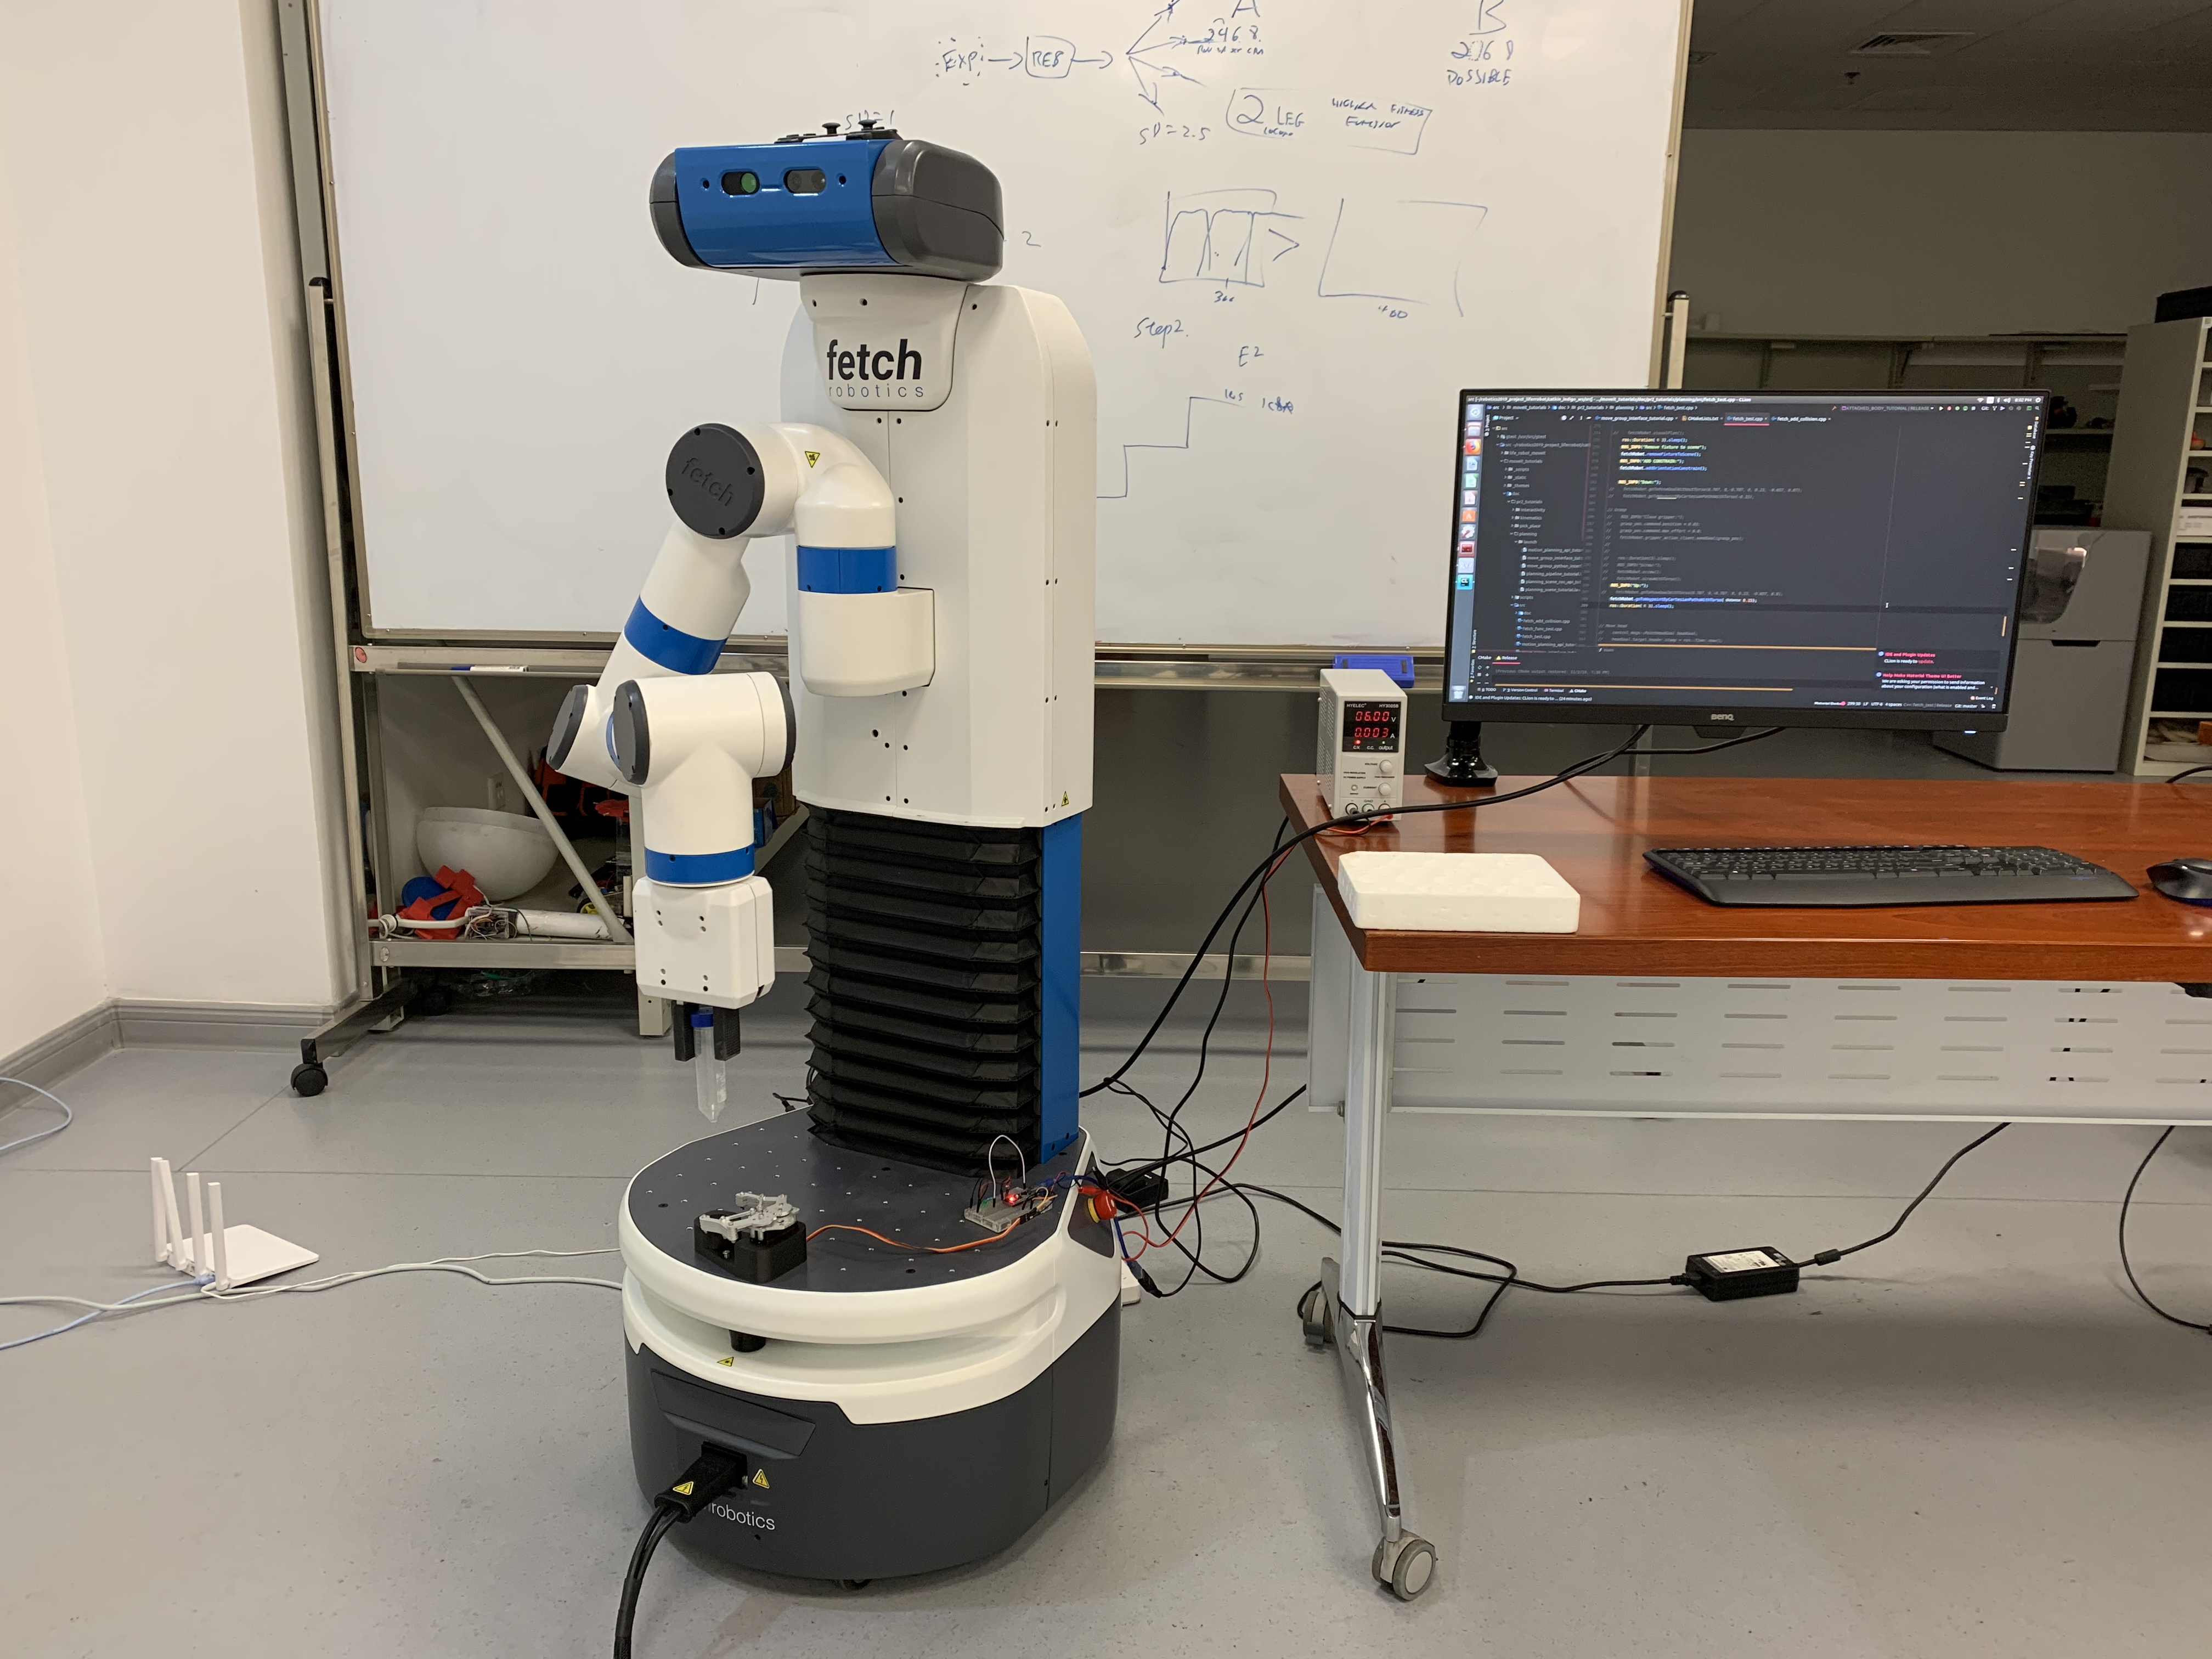
\includegraphics[width=0.3\textwidth]{img/p6.jpg}
    }
    \caption{Steps of grasping the centrifuge tube.}
    \label{movement}
    \end{figure}
    
	We choose four criteria to evaluate the performance.
	\begin{itemize}
		\item  Localization accuracy\\
		In the beginning, the Fetch robot needs to move to the place where it grasps the centrifuge tube. There are two ways to evaluate the localization accuracy. 1. We can use the data from the tracing system as the ground truth and compare it with the data from amcl. 2. We add another QR code on the table, and obtain the transform from table to robot, and use this data compare with the data from amcl.
		\item Success rate of grasping and placing\\
				After the robot moves to the designated position, it needs to grasp the tube and place it on its fixed platform. We can do it in 50 attempts and see how many times it successfully grasps and places the tube.
		\item Alignment error\\
		Because the centrifugal tube has a lid, and in this experiment, it is necessary to screw the lid and place it on the table, then grasp the lid and re-screw it back on the tube. At this point, the alignment error between the lid and the tube is involved. We can evaluate the performance of the manipulator by measuring the eccentricity distance between the lid and the tube.
		\item Task time\\
		In this experiment, we use different IK methods to test the time required for the robot to complete the whole tasks and a shorter time means better performance.
		
	\end{itemize}
	
	\section{Conclusions}
	%Short summary and conclusions. Including future work (things that should/could be done to improve the system).
	In this project, we have proposed a method for labware transportation and dexterous manipulation of centrifuge tubes in life science laboratories using a Fetch robot. Also, we are planning to adopt another pose estimation method, DenseFusion for object recognition. Both methods will work in the experiment while DenseFusion might perform better than AprilTag because of the unrestricted shape of labware containers. In the future, the development of repeatable and simple experiments in life science laboratories, very often plagued with manual transportation, could profit from this.
	
	
	% use section* for acknowledgment
	%\section*{Acknowledgment}
	% optional entry into table of contents (if used)
	%\addcontentsline{toc}{section}{Acknowledgment}
	%The preferred spelling of the word "acknowledgment" in America is
	%without an "e" after the "g." Try to avoid the stilted expression,
	% "One of us (R. B. G.) thanks..." Instead, try "R.B.G. thanks..." Put
	% sponsor acknowledgments in the unnumbered footnote on the first
	% page.
	
	% trigger a \newpage just before the given reference
	% number - used to balance the columns on the last page
	% adjust value as needed - may need to be readjusted if
	% the document is modified later
	%\IEEEtriggeratref{8}
	% The "triggered" command can be changed if desired:
	%\IEEEtriggercmd{\enlargethispage{-5in}}
	
	
	\bibliographystyle{ieeetr}%{splncs04}
	\bibliography{ref}
	
	
\end{document}
